\documentclass[
		a4paper,     % Format A4       
        twoside,     % zweiseitig %TODO undo
        BCOR10mm,    % binding correction
        cleardoubleempty, % empties cleardoublepage    
        parskip,     % Abstand zwischen Abs‰tzen, statt Einr¸ckung
        headsepline,  % separate heading and text by a line
        titlepage,   % mit Titelseite
        bibtotoc,    % include bibliography in TOC
%				liststotoc,
%       draft,       % renders faster, shows overfull boxes, doesn't render images
]{scrartcl}

% packages
\usepackage[ngerman, english]{babel} % choose your language with \selectlanguage{}
\usepackage[T1]{fontenc}
\usepackage[utf8]{inputenc} % ansinew avoids escaping german umlauts

\usepackage{verbatim}
\usepackage{graphicx} % graphics can be included using \includegraphics{}
\usepackage{iflang}
\usepackage{textcomp}
\usepackage{amsmath,amssymb}
\usepackage{hyperref}
\usepackage{listings}
\usepackage{blindtext}
\usepackage{enumitem}
\usepackage{tikz}
\usepackage{caption}
\usepackage{float}
\usepackage{xcolor}
\usetikzlibrary{shapes,arrows, positioning, backgrounds, chains}

%\captionsetup[figure]{justification=raggedright, singlelinecheck=false} 


% !BIB program = bibtex

% additional settings
\hypersetup{
 	pdfauthor={},
 	pdftitle={},
 	pdfsubject={Bachelor Thesis}, 
 	pdfkeywords={}
 	colorlinks=true,        % false: boxed links; true: colored links
 	linkcolor=black,        % color of internal links
	citecolor=black,        % color of links to bibliography
	filecolor=black,        % color of file links
	urlcolor=black          % color of external links
}

% stretch text vertically by factor (zeilenabstand)
\renewcommand{\baselinestretch}{1.150}\normalsize
\newcommand{\footurldated}[2]{\footnote{\url{#1} (Abgerufen: #2)}}
\newcommand{\code}[1]{\texttt{#1}}


% avoid single lines at beginning/end of page
\clubpenalty10000
\widowpenalty10000

% custom hyphenation
\hyphenation{
% Ma-na-ge-ment  Netz-werk-ele-men-ten
% Netz-werk Netz-werk-re-ser-vie-rung
	BPMN---Community
}

\addtokomafont{sectioning}{\rmfamily}

% set path to image directory
\graphicspath{{images/}}

\lstset{
   basicstyle=\small,
   tabsize=4,
   showspaces=false, 
   showstringspaces=false, 
}

\tolerance=6000
\setlength{\emergencystretch}{3.0em}
\parskip8pt

\renewcommand{\descriptionlabel}[1]{
\normalfont\bfseries #1:}


% Replace with your information
\newcommand{\Author}{Lukas Hüller}
\newcommand{\TitleGerman}{Konzeption einer Datenspeicherlösung zur Erstellung von RPA-Robotern in verschiedenen Modellierungsoberflächen}
\newcommand{\TitleEnglish}{Design of a data storage solution for the creation of RPA robots in different modeling interfaces}

\addto\extrasenglish{
	\renewcommand{\sectionautorefname}{Chapter}
	\renewcommand{\subsectionautorefname}{Section}
	\renewcommand{\subsubsectionautorefname}{Section}
	\renewcommand{\figureautorefname}{Fig.}
	\def\lstlistingautorefname{Listing}
}


\begin{document}
% 	\selectlanguage{english}
	\selectlanguage{ngerman}

	\IfLanguageName{ngerman}{
		\def\sectionautorefname{Kapitel}
		\def\subsectionautorefname{Abschnitt}
		\def\subsubsectionautorefname{Abschnitt}
		\def\figureautorefname{Abb.}
		\def\lstlistingautorefname{Listing}
		\renewcommand{\refname}{Quellenverzeichnis}}{
	}

	% special pages	
	\begin{titlepage}
	\begin{flushright}
		
\includegraphics[height=.15\textheight]{uni_logo.eps}
		\hfill
		
\includegraphics[height=.15\textheight]{hpi_logo.eps}
	\end{flushright}
	\begin{center}
		\hbox{}
		\vfill
		\IfLanguageName{ngerman}{
			{\huge\bfseries\TitleGerman\par}
			\vskip 0.3cm
			{\textit{\TitleEnglish\par}}
		}{
			{\huge\bfseries\TitleEnglish\par}
			\vskip 0.3cm
			{\slshape\TitleGerman\par}
		}
		\vskip 1.5cm
		\textbf{\Author}\\
		\vskip 1.7cm
		\begin{tabular}{l}
			Prof.~Dr.~Mathias~Weske \\
			Maximilian Völker,~MSc. 
		\end{tabular}
		\vskip 0.25cm
		\begin{tabular}{l}
			\IfLanguageName{ngerman}{
				Fachgebiet für Business Process Technology
			}{
				Business Process Technology Group
			}
		\end{tabular}
		\vskip 1.5cm
		\begin{tabular}{ll}
			\IfLanguageName{ngerman}{
				Datum der Abgabe:
			}{
				Date of Submission:
			} & 28.06.2021 \\
		\end{tabular}
	\end{center}	
	\vfill
\end{titlepage}


	\cleardoublepage
	\thispagestyle{empty}
\vspace*{24\baselineskip}
\hbox to \textwidth{\hrulefill}
\par
Ich erkläre hiermit, dass ich die vorliegende Bachelorarbeit selbstständig verfasst und keine anderen als die angegebenen Quellen und Hilfsmittel verwendet habe.

Potsdam, {\selectlanguage{ngerman}\today}
\newline
\newline
\newline
\newline
\newline
Lukas Hüller

\clearpage
	% \cleardoublepage
	% \thispagestyle{empty}
\vspace*{24\baselineskip}
\hbox to \textwidth{\hrulefill}
\par
I hereby affirm that I have written this bachelor's thesis independently, without using any sources other than those stated.

Potsdam, {\selectlanguage{english}\today}
\newline
\newline
\newline
\newline
\newline
Name

\clearpage
	\begin{abstract}
\textbf{Abstract.} 
Die Robotic Process Automation (RPA) hat in den vergangenen Jahren im Bereich der Automatisierungslösungen zunehmend an Bedeutung gewonnen. Der Markt stellt inzwischen eine Vielzahl von Plattformen zur Verfügung, mit denen die Automatisierungen erstellt werden können. Fast alle dieser Plattformen besitzen proprietäre Oberflächen zur Erstellung der Roboter, wodurch ein ständiges Übersetzen der modellierten und dokumentierten Prozesse aus bekannten Modellierungssprachen wie die Business Process Model and Notation (BPMN) oder Flowcharts in die Darstellungsform der Anwendungen notwendig ist. Dadurch erhöht sich der Aufwand für RPA-Entwickler und Prozessexperten in der Erstellung der Roboter. 

Die vorliegende Arbeit untersucht die für die Erstellung von RPA-Robotern geeigneten Notationen. Auf dieser Grundlage wird eine Architektur vorgestellt, die das Speichern der Roboter in einer einheitlichen Datenspeicherlösung ermöglicht. Zudem wird gezeigt, wie die verschiedenen Repräsentationen aus dieser \textit{\glqq Single Source of Truth\grqq{}} (SSoT) generiert werden können. Mit der vorgestellten Lösung ist es möglich, RPA-Roboter in verschiedenen Modellierungssprachen zu erstellen. Dadurch werden Prozessexperten sowie Low-Code-Developer in die Lage versetzt, direkt in ihrer gewohnten Modellierungsumgebung die Automatisierungen zu programmieren.

\end{abstract}
	\cleardoublepage
	
	% listings
	\pagenumbering{Roman}
	\tableofcontents
	\listoffigures
	\listoftables
	\cleardoublepage
	
	% include your chapters
	\pagenumbering{arabic}
	\section{Einführung}
\label{sec:ein}

Unternehmen stehen unter immensem Druck, ihre Prozesse und Abläufe zu automatisieren. Oftmals ist die Robotic Process Automation, die in den vergangenen Jahren ein beeindruckendes Wachstum erfährt \cite{GartnerQuadrant},  hierfür die geeignete Automatisierungsstrategie. RPA steigert die Produktivität der Abläufe durch den Einsatz sogenannter Softwareroboter. Diese Roboter übernehmen die Aktivitäten des Nutzers in Desktop- oder Webanwendungen, indem sie seine Interaktion mit den Oberflächen eigenständig ausführen. Da in den automatisierten Prozessen lediglich die menschlichen Softwareanwender durch den Menschen imitierende Roboter ersetzt werden, bleibt der Prozess unverändert. Dadurch entfällt der hohe Aufwand der Prozessintegration. 

Durch das große Wachstum dieser Automatisierungstechnologie entstand eine Vielzahl von Plattformen, die das Erstellen der Softwareroboter ermöglichen. Jedoch haben die mit potenziellen Stakeholdern durchgeführten Interviews gezeigt, das Funktionen gewünscht werden, die keine auf dem Markt verfügbare Plattform abbildet.
Wie im Fazit auf der Seite \pageref{anforderungsanalyse:fazit} detailiert beschrieben, dominierte in den Interviews der Wunsch nach einer RPA-Plattform, mit der Roboter durch verschiedene, standardisierte Modellierungssprachen wie zum Beispiel der BPMN, der Flussdiagramm-Syntax oder als Ereignisgesteuerte Prozesskette (EPK) erstellt werden können. Dies soll das Konfigurieren der Roboter für Low-Code-Entwickler\footnote{Low-Code-Entwickler\\ Entwickler, die vor allem mit grafischen Programmieroberflächen wie z. B. Blockeditoren oder Modellierungssprachen anstatt von textbasierter Programmierung arbeiten.} ermöglichen. Alle in der Branche bekannten Plattformen unterstützten lediglich das Modellieren von Robotern in deren proprietären Oberflächen; standardisierte Notationen können bislang nicht zum Erstellen einer Automatisierung verwendet werden. 

In der ersten Forschungsfrage dieser Arbeit wird untersucht, ob sich Modellierungssprachen zur Erstellung von RPA-Robotern eignen. In der zweiten Forschungsfrage wird analysiert, wie das Erstellen desselben Roboters in verschiedenen Modellierungssprachen erfolgen kann, sodass jeder an der Automatisierung beteiligte Entwickler die ihm vertraute Modellierungssprache verwenden kann. Hierzu werden eine einheitliche Speicherlösung für RPA-Roboter sowie die zur Übersetzung in visuelle Repräsentationen notwendigen Parser vorgestellt.

Nach einer Einführung in die RPA, einem Überblick über verwandte Arbeiten sowie der Dokumentation der Befragungen, wird im Kapitel \ref{analyse_sprachen} untersucht, ob sich Modellierungssprachen  für die Entwicklung von RPA-Robotern eignen. Auf Grundlage dieser Betrachtungen ist im nachfolgenden Kapitel das Konzept der einheitlichen Speicherlösung beschrieben. Das Kapitel \ref{implementierung_ssot} erklärt, wie die beschriebenen Konzepte implementiert werden können. Abschließend werden die Implementierung evaluiert (Kap. \ref{evaluation_ssot}), die wesentlichen Erkenntnisse zusammengefasst sowie ein Überblick über offene Forschungsfragen (Kap. \ref{conclusion}) gegeben. 
 
	\clearpage
	
	\section{Grundlagen}

Dieses Kapitel führt detailliert in die Robotic Process Automation ein und zeigt die Vorteile dieser Automatisierungsmethode auf. Zudem werden verwandte Arbeiten vorgestellt, die sich mit den Themen der Robotermodellierung in bekannten Notationen oder der einheitlichen Speicherung von Robotermodellen befassen.

\subsection{Einleitung zur Robotic Process Automation}


In den vergangenen Jahrzehnten wurde das Workflow Management angewendet, um Arbeitsabläufe computergestützt zu automatisieren \cite{Aalst2004}. Ein großes Problem bei der Einführung des Workflow Managements stellt die meist mangelhafte Akzeptanz der Mitarbeiter dar. Ebenso lassen sich vollständige Automatisierungen nur schwer in bestehende Systeme integrieren. Um diesen Problemen vorzubeugen, wird das Workflow Management seit einigen Jahren um das Business Process Management (BPM) ergänzt \cite{Aalst2021}. BPM legt den Schwerpunkt auf die von den Mitarbeitern ausgeführen Aufgaben und ermöglicht durch die verwendete Notation BPMN eine vereinfachte Analyse und Optimierung des Prozesses. Da die Mitarbeitenden bei den Automatisierungen nun stärker im Fokus stehen, steigt die Akzeptanz derer bei der Einführung der Automatisierungslösung. Jedoch wird der BPMN vorgeworfen, durch den verstärkten Einsatz der Modellierung den zu automatisierenden Prozess aus dem Fokus zu verlieren. \glqq Schlussendlich ist das Ziel nicht die Modellierung, sondern die Verbesserung des existierenden Prozesses\grqq{} \cite{Aalst2004}.

Um dem meist kostspieligen BPM mit den genannten Nachteilen entgegenzuwirken, wird seit einigen Jahren die Robotic Process Automation entwickelt. Sie wurde anfangs von Wirtschaftsunternehmen vorangetrieben und gerät nun seit vielen Jahren in den Fokus der Wissenschaft \cite{AalstProcessMining}. Ziel der RPA ist es, die vom Nutzer in Drittanwendungen ausgeführten Schritte zu erkennen, aufzuzeichnen und nachfolgend automatisiert auszuführen. Dabei interagiert der sogenannte Softwareroboter analog zum Nutzer mit der grafischen Oberfläche der Software. Da RPA direkt auf dieser Anwendungsebene arbeitet, fällt der Integrationsaufwand im Vergleich zu anderen Automatisierungsmethoden deutlich geringer aus. Es kann weiterhin die bestehende Software genutzt werden, es müssen keine offenen Schnittstellen entwickelt oder gar neue Hardware angeschafft werden. Zwingend notwendig sind jedoch eindeutig definierte Aufgabenfolgen. So lassen sich mittels RPA zum Beispiel Formulare ausfüllen, Daten verschieben, Mails versenden aber auch Informationen von Webseiten verarbeiten. 

RPA ist eine weltweit bekannte Technologie und wird bereits in zwei Dritteln der deutschen Unternehmen verwendet \cite{isgRPA} \cite{pwcRPA}. Zudem ist die RPA mit 63~\% Wachstum in 2018 das am schnellsten wachsende Segment der Softwareentwicklung \cite{gartner}. Ebenso zeichnet sich die Technologie durch eine schnelle Kapitalrendite aus, die vor allem durch den Bottom-Up Ansatz begründet wird. \glqq Oftmals werden die vollständigen Prozesse betrachtet, jedoch nur kleinere Gruppen von Aufgaben - die sogenannten \frqq Quick-wins\flqq - direkt automatisiert \cite{aalstYoutube}.\grqq{} Dies ist nur dadurch möglich, da die Roboter „Hand-in-Hand“ mit den Anwendern arbeiten. 

Wie eingangs beschrieben, unterstützt BPM das Workflow Management bei der Prozessoptimierung. Zur Verbesserung der bestehenden Prozesse wird im Vorfeld einer Robotic Process Automation das Process Mining verwendet. Process Mining analysiert Geschäftsprozesse durch das Verarbeiten und Korrelieren von Datenströmen. Es erkennt Muster in den Prozessdaten und hilft somit das Verständnis der Prozesse zu verbessern. Dadurch lassen sich Möglichkeiten für die sinnvolle Einbindung von RPA erkennen. Vor der Implementierung einer RPA-Lösung empfiehlt sich eine Analyse des umzusetzenden Prozesses mittels Process Mining, da andernfalls der Prozess zwar automatisiert, jedoch vorher nicht optimiert wird. 

Bekannte RPA-Plattformen entwickeln unter anderem die Firmen \mbox{UiPath}\footnote{https://www.uipath.com/de/ (Abgerufen 12. Juni 2021)}, \mbox{blueprism}\footnote{https://www.blueprism.com/de/ (Abgerufen 12. Juni 2021)} und \mbox{AutomationAnywhere}\footnote{https://www.automationanywhere.com/de/ (Abgerufen 12. Juni 2021)}. Die Firma Microsoft stellt mit \code{Power Automate Desktop} seit März 2021 ihre eigene kostenlose RPA-Plattform zur Verfügung. Einige der Plattformen - wie zum Beispiel UiPath - besitzen ein ausgeprägtes \code{Recoding-Feature}, mit dem die zu automatisierenden Aufgaben direkt aufgenommen werden können. Andere hingegen lassen sich  einfacher bedienen oder unterstützen eine Vielzahl an Drittanwendungen. 

\subsection{Einleitung zu Modellierungssprachen}

Um Organisationsstrukturen, Software aber auch Prozesse zu skizzieren, werden zur Beschreibung der Sachverhalte visuelle Modellierungssprachen verwendet \cite{winter2000}. \glqq Neben der Unterstützung bei der Erfassung und Dokumentation sind diese graphischen und textuellen Beschreibungsmittel auch wesentliche Hilfsmittel zur Kommunikation bei der (Weiter-) Entwicklung von Organisationen und Softwaresystemen\grqq{}, beschreibt A. Winter den Nutzen von Modellierungssprachen treffend. Modellierungssprachen unterscheiden sich in dem zur Verfügung gestellten „Vokabular und der Grammatik“, mit der Sachverhalte der menschlich wahrgenommenen Realität in Modellen abgebildet werden können \cite{Fleischmann2018}.

In der durch die Object Management Group (OMG) standardisierten Unified Modeling Language (UML) ist eine Sammlung von Notationen definiert. Die UML umfasst unter anderem das in der Objektmodellierung bekannte Klassendiagramm, das für die Funktionsmodellierung genutzte Use Case Diagramm oder auch das Komponentendiagramm zur Beschreibung von IT-Systemstrukturen. Für dieses Werk von Relevanz sind  die Notationen zur Prozessmodellierung. Diese Sprachen dienen der Darstellung von Interaktionsschritten innerhalb eines Prozesses und eignen sich daher unter Umständen auch zur Modellierung von RPA-Robotern. Bekannte Vertreter sind hierbei das Datenfluss-orientierte Flussdiagramm, die Kontrollfluss-orientierten Sprachen wie die BPMN, das Petri-Netz oder auch die ereignisgesteuerte Prozesskette \cite{mastersthesisLobe}.

\subsection{Verwandte Arbeiten}

In der bestehenden Literatur sind nur wenige Ansätze von Untersuchungen oder Prototypen für die Erstellung von RPA-Robotern in Modellierungssprachen zu finden. Dies ist sehr verwunderlich, da zahlreiche Artikel \cite{alejandro}\cite{rpameetsbpmn} die Wichtigkeit der Dokumentation und Prozessanalyse im Zusammenspiel mit RPA erwähnen.

\clearpage

Eine interessante Arbeit ist womöglich die Abschlussarbeit des Studenten Johann Schäfer der FH Münster \cite{Viadee}. Leider erhielt ich auch nach mehreren Kontaktversuchen keine Antwort auf die Anfrage, die Abschlussarbeit oder vielleicht sogar das Softwareprojekt betrachten zu dürfen. Daher war eine qualitative Analyse sowie eine aufbauende Forschung auf den Erkenntnissen der Arbeit des Studenten nicht möglich.

Der Autor beschreibt eine Weiterentwicklung des \code{bpmn-io} BPMN-Modelers, die sich zum Erstellen von RPA-Robotern eignen soll. Wie in Abbildung \ref{fig:viadee} zu sehen, ist es möglich, mit der entstandenen Plattform jeder BPMN Service Task eine RPA-Aufgabe zuzuweisen. In den grünen Boxen unterhalb der Task ist es möglich, der Aufgabe Parameter zu übergeben. Zudem wird ein aufklappbarer Subprozess verwendet, um auch kleinteilige Automatisierungsschritte übersichtlich darzustellen. Im Hauptprozess (oben dargestellt) ist durch die Annotation direkt erkenntlich, welche Teile des Prozesses mittels RPA automatisiert werden.

\begin{figure}[h!]
    \centering
    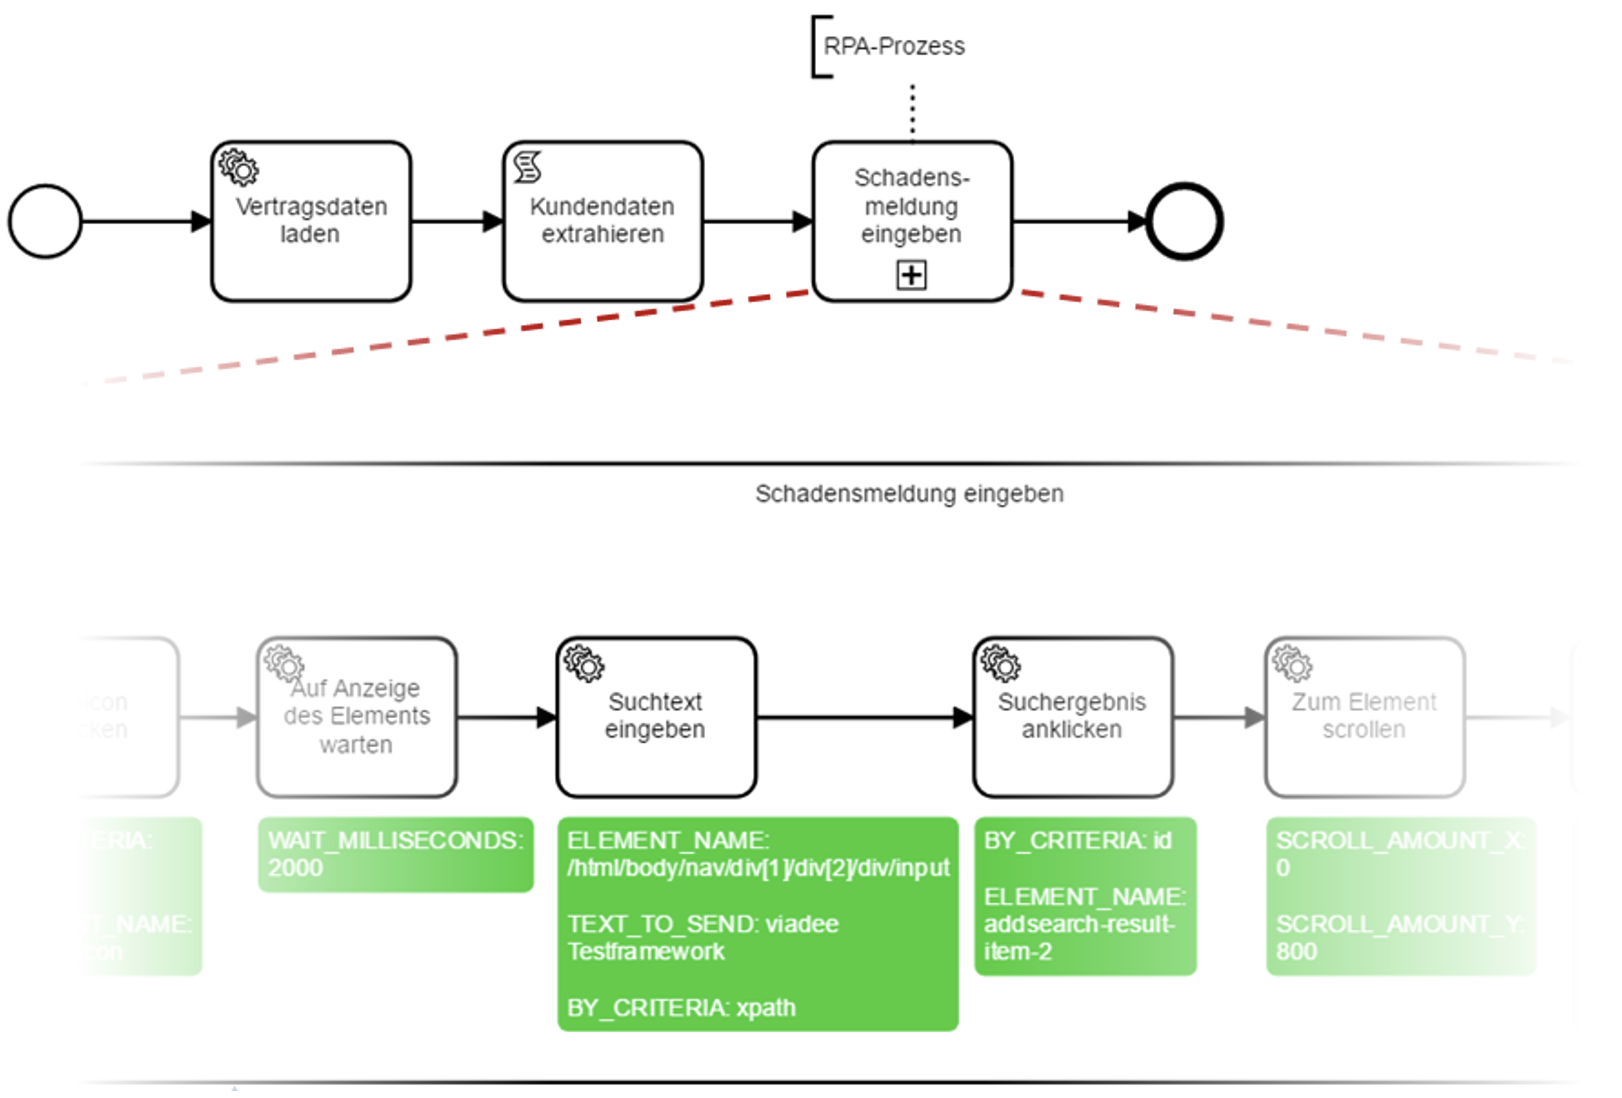
\includegraphics[width=1.0\textwidth]{Bachelorarbeit/images/ScreenshotRelatedWork3.png}
    \caption{Screenshot der Modellierungsoberfläche des viadee-Roboters}
    \label{fig:viadee}
\end{figure}

	\clearpage
	
	\section{Anforderungen an eine RPA-Plattform} \label{anforderungsanalyse}

UiPath veröffentlichte 2018 eine Auflistung \cite{uiPathReq} von sieben Anforderungen, die eine moderne RPA-Plattform erfüllen sollte. Da die Veröffentlichung bereits einige Jahre zurückliegt und die Entwicklung der RPA-Plattformen stetig voranschreitet, wurden zu Beginn des Projektes verschiedene Stakeholder befragt. Ziel der elf Interviews war es, die Anforderungen an eine neue RPA-Plattform zu definieren und mit den Ergebnissen der UiPath-Studie abzugleichen. 

In der nachfolgenden Zusammenfassung werden die für diese Arbeit relevanten Informationen zur Interaktion der Stakeholder mit den Modellierungsoberflächen hervorgehoben.

\subsection{Dokumentation der Interviews}
\label{interviews}

In den Interviews wurden neben Lehrstuhlmitarbeitenden, die unter anderem an Themen rund um RPA forschen, Prozessexperten, vier RPA-Entwickler\footnote{RPA-Entwickler \\ haben auch beratende Funktionen, weshalb die Begriffe RPA-Consultant und RPA-Developer von nun an synonym verwendet werden.} sowie ein Manager befragt. Als Prozessexperten wurden aus der Verwaltung des Hasso-Plattner-Instituts eine Sekretärin zweier Fachgruppen sowie die Referentin für Forschung und Lehre interviewt. Als IT-Prozessexperte wurde ein Experte für Vulnerability Management des Cyber Defence Centers der Deutschen Telekom befragt, der seit über einem Jahr mit einem externen Team an softwaregestützten Prozessautomatisierungen arbeitet. Zudem wurde der General Manager und Chief Financial Officer (CFO) von Thermondo interviewt.

\clearpage
\subsubsection{Interview: Prozessexperten aus der Verwaltung}
Die Prozessexperten der Verwaltung betonten, dass es in ihrem Büroalltag einen großen Bedarf für die Automatisierung und Digitalisierung von Prozessen gibt. Die tägliche Arbeit ist zwischen einem und zwei Dritteln von monotonen Verwaltungsaufgaben dominiert, die den Angestellten weder Spaß bereitet, noch sie im gewünschten Umfang bei der Arbeit effektiv voranbringt. Es wurden zahlreiche Prozesse vorgestellt, die wiederkehrend und auch fehleranfällig sind. Leider sind viele dieser Prozesse nur teilweise digitalisiert, weshalb eine End-To-End-Automatisierung mittels RPA vorab eine Digitalisierung der Prozesse erfordert.

\subsubsection{Interview: Prozessexperten in IT-Projekten}
Der Cyber Defence Experte arbeitet seit sechs Monaten als Prozessexperte mit zwei externen Entwicklern zusammen, die für ihn alltägliche Routineaufgaben automatisieren. Er bemängelte, dass der Erstellungsprozess der Roboter sehr viel Zeit in Anspruch nimmt. Zu Beginn jedes Automatisierungsprojektes erläutert er den Entwicklern und Consultants welche Prozesse automatisiert werden sollen. Auf dieser Grundlage wird mit allen Beteiligten ein Programmablaufplan erstellt. Im Anschluss daran entwickeln die Consultants die Automatisierung mit ihrer Plattform und präsentieren den Roboter dem Kunden. Dieser hat abschließend jedoch keinen Zugriff auf die Automatisierung, was er bemängelt. Ebenso würde der Prozessexperte gern kleine Änderungen an den fertigen Automatisierungen in einem leicht zu bedienen Interface direkt vornehmen können. Auch dies ist mit den derzeit bestehenden Lösungen nicht möglich.

\subsubsection{Interview: RPA-Entwickler}
In umfangreichen Interviews wurden vier RPA-Developerbefragt, die  mehrjährige Erfahrung im Bereich der RPA besitzen. 

Die Entwickler arbeiten seit einigen Jahren mit der Software des Marktführers UiPath. Der Prozess zur Erstellung eines Softwareroboters beginnt mit der Prozessvorstellung durch den Kunden. Im Nachgang des Erstgespräches werden die Prozesse detailliert gezeichnet. Hierzu wird von den Befragten ausschließlich die Modellierungssprache BPMN verwendet.  Auf Grundlage der Prozessskizze wird mögliches Potenzial zur Optimierung der Abläufe analysiert, bevor es zur finalen Besprechung mit dem Kunden erfolgt. Danach beginnt die Implementierung des Roboters in UiPath. Hierbei merkten beide Entwickler an, dass das gedankliche Übersetzen eines in BPMN gezeichneten Prozesses in die proprietäre UiPath-Syntax unnötig kompliziert ist. Aus ihrer Sicht sollte es auch möglich sein, einen RPA-Roboter direkt in der BPMN-Syntax zu erstellen. Einer der  Entwickler sagte zudem, dass nach Fertigstellung des Roboters dieser noch dokumentiert werden muss. Dafür eignet sich seiner Meinung nach BPMN als Dokumentationssprache hervorragend. Da der final implementierte Roboter oftmals von der ursprünglichen Skizze abweicht, muss dieser zu Dokumentationszwecken erneut in BPMN skizziert werden. Gewünscht wurde auch eine Dokumentationshilfe, die die verwendeten RPA-Befehle direkt in die Dokumentation einfließen lässt. Solch eine Funktion sucht man bisher auf dem Markt vergeblich. 

Ebenso merkten zwei Entwickler an, dass die Oberfläche von UiPath sehr komplex und benutzerunfreundlich ist. Zwei Entwickler suchen daher seit langer Zeit nach einem Tool, dass sich leichter bedienen lässt. Leider umfassen diese Tools meist nicht alle benötigten Funktionen, weshalb schlussendlich doch wieder auf UiPath zurückgegriffen werden muss. 

Weiterhin wurde von einem Entwickler ein "Marktplatz"  für Roboter gewünscht, der es ermöglichen sollte, Roboter innerhalb der Organisation oder auch in einer Open-Source Community zu teilen. Zudem sollte es eine Administrationsoberfläche geben, von der aus zentral Aktualisierungen eingespielt werden können. 

\subsubsection{Interview: Manager \& CFO}
Seit mehreren Jahren ist der Manager bestrebt, analoge Prozesse im Heizungs- und Handwerkerwesen zu digitalisieren. Er hofft, dass seine Firma durch eine höhere Anzahl automatisierter Prozesse in Zukunft besser skalieren kann. Seine wichtigste Feststellung aus den vergangenen Jahren war, dass man in Deutschland meilenweit von vollständig „automatisierbaren“ Prozessen entfernt ist. Der Grund hierfür sei, dass sich softwarebasierte Prozesse aufgrund veralteter Software und somit fehlender Schnittstellen (APIs) nicht automatisieren lassen. Er zeigte sich begeistert von der für ihn unbekannten Zukunftstechnologie RPA und wünschte sich eine Plattform, mit der auch Prozessexperten Roboter erstellen können. Der Manager betonte, dass viele Bestrebungen nach verstärkter Automatisierung nicht nur an fehlender Digitalisierung scheitern. \glqq Entwickler und Prozessberater sind schlichtweg zu teuer\grqq{}, verriet der CFO.

\subsection{Fazit}
\label{anforderungsanalyse:fazit}
Die vielfältigen Antworten der Befragten waren grundlegend für die Definition der Anforderungen an die neue Plattform. Zusammenfassend lässt sich festhalten, dass in allen Branchen, die die Befragten repräsentieren, ein ausgesprochen großes Interesse an den Möglichkeiten der Automatisierung bestand, um die alltägliche Arbeit zu erleichtern und zu effektivieren. 
Die Mitarbeitenden der Verwaltung sagten uns, dass bei der Entwicklung der Plattform in jedem Fall ein besonderes Augenmerk auf die alltagstaugliche Bedienung und schnelle Erlernbarkeit gelegt werden sollte. Die RPA-Developer wünschten sich vor allem eine leicht zu bedienende RPA-Plattform, mit der bestenfalls direkt in BPMN Roboter skizziert, Automatisierungen erstellt und abschließend die Prozesse dokumentiert werden können. Thermondos CFO verdeutlichte, dass mit einer guten RPA-Plattform auch Prozessexperten Roboter erstellen können sollen. \glqq Die Kosten für RPA-Consultants sind für viele Firmen eine Herausforderung\grqq{}, so der Manager. 

Die Auswertung der Interviews zeigt, dass sich der Großteil der Anforderungen aus der UiPath-Studie in den aktuellen Wünschen der Entwickler wiederspiegelt. Die Studie erachtet es als zwingend notwendig, dass die Roboter durch die Mitarbeitenden der Fachabteilungen erstellt werden können. Ebenso erwähnt die Veröffentlichung die Anforderung eines Marktplatzes für Roboter, mit der die \glqq globale Anwender-Community\grqq{} von den fertiggestellten Automatisierungen profitiert. Die Auflistung von UiPath bestätigt die Notwendigkeit eines Administrations-Interfaces und beschreibt zudem noch die Management-Konsole, die es den Mitarbeitern erleichtern soll, die Automatisierungen zu starten, zu kontrollieren und zu validieren. Einzig die Nutzung von Künstlicher Intelligenz, die als eine Anforderung von UiPath beschrieben wurde, konnte nicht aus den Interviews abgeleitet werden.
	\clearpage
	
	\section{Analyse geeigneter Prozessmodellierungssprachen}\label{analyse_sprachen}

„Von der Wahl der Modellierungssprache hängt also ab, was in einem Modell überhaupt abgebildet werden kann, und was nicht sichtbar werden kann, weil die Modellierungssprache keine Konzepte dafür anbietet.“ \cite{Fleischmann2018} Die Interviews ergaben die Notwendigkeit der Funktion, RPA-Roboter in Modellierungssprachen zu erstellen. Daher wird nachfolgend untersucht, welche Notationen sich für die Implementierung von RPA-Robotern eignen. 

\subsection{Analyse des ausführbaren RobotFramework Codes}

Betrachten wir vor der Analyse der Modellierungssprachen die Syntax der Programmiersprache RobotFramework\footnote{\url{www.robotframework.org} (Abgerufen 19. Juni 2021)}, um im Anschluss bewerten zu können, welche Programmierkonzepte von den Notationen unterstützt werden müssen. RobotFramework wurde für die Ausführung der Automatisierungen gemeinsam mit den Bibliotheken des RpaFrameworks\footnote{\url{www.rpaframework.org} (Abgerufen 19. Juni 2021)} verwendet. 

RobotFramework ist ein quellenoffenes Framework, das für die Testautomatisierung und RPA verwendet werden kann. Es bietet einen leicht lesbaren Code, mit dem auch Einsteiger Automatisierungen erstellen können. Das Framework wird aktiv weiterentwickelt und von zahlreichen Unternehmen wie beispielsweise DB~Schenker,  Capgemini, Kuka oder auch der Deutschen Post verwendet. Alle zugrunde liegenden Bibliotheken sind in Java oder Python implementiert und können daher bei Bedarf erweitert werden.\footnote{sämtliche Informationen entnommen aus: \\ \url{https://robotframework.org/\#introduction} (Abgerufen 19. Juni 2021)}

Die Bibliotheken des \mbox{RpaFrameworks} stellen die RPA-Aufrufe zur Verfügung. Die zugrunde liegende Programmierlogik wird in der Syntax der Test-Entwicklungssprache \mbox{RobotFramework} geschrieben. Daher wird sich im Verlauf der Arbeit vor allem auf diese Syntax bezogen. 

RPA-Roboter beschreiben Nutzerinteraktionen in verschiedenen Desktopanwendungen oder Browsern. Da es sich bei den Automatisierungen um ausführbare Programme handelt, besitzen diese die typischen Elemente einer jeden Programmiersprache. Somit finden sich in RobotFramework sequenzielle Anweisungen, Verzweigungen sowie terminierte Wiederholungen (implementiert als \code{FOR}- oder \code{WHILE}-Schleife). Zudem werden in RobotFramework Variablen unterstützt. Oftmals werden diese genutzt, um das Ergebnis einer RPA-Aktivität (zum Beispiel \flqq Microsoft Excel\frqq $\rightarrow$ \frqq Get Cell Value\flqq) zwischenzuspeichern und dann als Eingabeparameter einer anderen Aktivität anzugeben. Die Konzepte von Try-Catch Blöcken sind aktuell noch nicht vollumfänglich implementiert und werden daher in dieser Arbeit nicht weiter betrachtet.

Anhand eines Beispiel-Roboters, der den elektronischen Versand eines Mahnbescheides automatisiert, werden nachfolgend die theoretischen Grundlagen erläutert. Dem Roboter zugrunde liegt eine EXCEL-Tabelle, die täglich von den Mitarbeitenden der Verwaltung gefüllt wird und den Vor- und Nachnamen des Kunden, die Mail-Adresse sowie den Mahnungszähler 1 oder 2 beinhaltet. Die letzte Zahl gibt an, die wievielte Zahlungsaufforderung an den Kunden gesendet werden soll. Der Roboter öffnet jede Nacht die erstellte EXCEL-Tabelle und geht Zeile für Zeile die Einträge der Tabelle durch.\footnote{Das automatische Starten des Roboters wird aus Komplexitätsgründen nicht betrachtet.} Er ließt dafür jede Zeile einzeln ein und prüft im Anschluss den Mahnungszähler. Abhängig von der eingetragenen Zahl wird er nun eine Mail an den Kunden erstellen und mit dem entsprechenden Mahnbescheid als Anlage versehen. Sobald der Roboter am Ende der Tabelle angekommen ist, terminiert die Automatisierung und das Mail-Programm schließt sich. 

\begin{table}[h!]
    \centering
    \caption{Ausgangstabelle des Beispielprozesses}
    \begin{tabular}{|l|l|l|c|}
    \hline
    \textbf{Lastname} & \textbf{Firstname} & \textbf{Mail}      & \textbf{Counter} \\ \hline
    Stella        & Patricia         & p.stella@outlook.com       & 1                      \\ \hline
    Matthäus      & Clara            & familie-matthaeus@gmx.com  & 2                      \\ \hline
    Zenzi         & Mathis           & m.zenzi@web.de             & 1                      \\ \hline
    Reinhold      & Cornelia         & conny.reinhold@t-online.de & 1                      \\ \hline
    \end{tabular}
    \label{tab:exampleExcel}
\end{table}

Im Anhang ist der ausführbare Prozess in der Syntax des RobotFrameworks dargestellt (Abbildung \ref{fig:ScrRobotFr}). Dabei wurde an einigen Stellen auf die Verwendung von Test-Case Bezeichnungen, die im übrigen Code rosa eingefärbt sind, verzichtet. Diese Einschränkung war notwendig, da jeder Testcase einen eigenen Variablen-Scope bildet, sodass die  lokalen definierten Variablen in darauffolgenden Anschnitten nicht wiederverwendet werden können.

\subsection{Analyse der Semantik ausgewählter Notationen}

Um einen Roboter vollumfänglich in einer Modellierungssprache erstellen zu können, muss diese mindestens genau so mächtig wie die verwendete Sprache der Automatisierung (in unserem Fall RobotFramework) sein. Diese Mächtigkeit findet sich vor allem in Modellierungssprachen, die es ermöglichen, Softwareprogramme oder Geschäftsprozesse abzubilden. In diesem Abschnitt werden die sehr verständlichen und aussagekräftigen Flussdiagramme \cite{WILHELM2007} sowie die BPMN, der meist eingesetzte Standard zur Abbildung von Geschäftsprozessen \cite{Fleischmann2018}, analysiert. Zudem werden die laut einer Studie zur Verbreitung von Notationen im deutschsprachigen Europa (\autoref{fig:survey} \cite{mastersthesisLobe}) sehr bekannten Ereignisgesteuerten Prozessketten (EPK) betrachtet. Diese sind jedoch kaum spezifiziert und werden daher außerhalb des deutschsprachigen Raumes nur selten verwendet \cite{Clemente2011}.

\begin{figure}[h!]
    \centering
    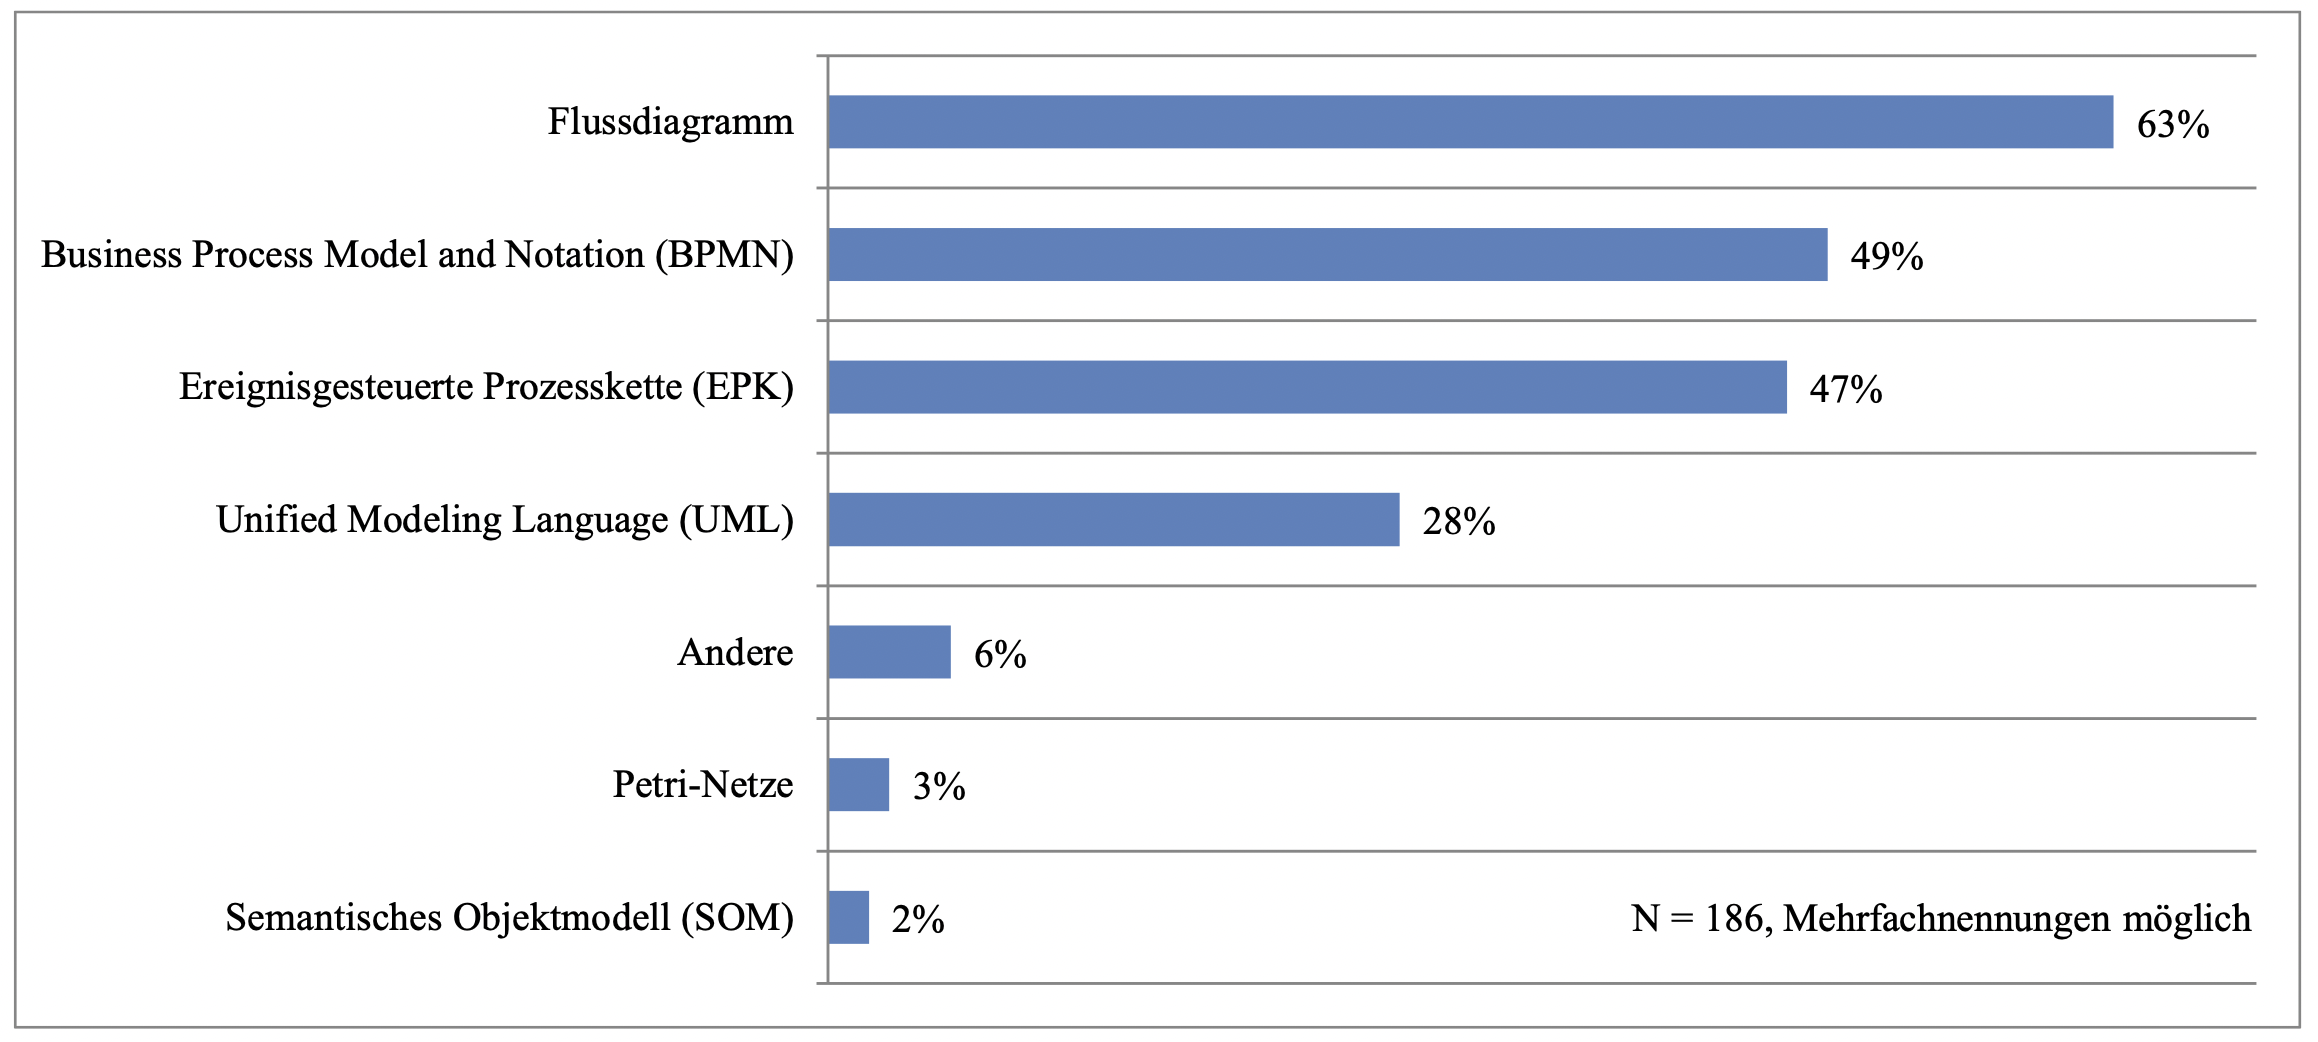
\includegraphics[width=1.03\textwidth]{images/studie_Modellierungssprachen.png}
    \caption{Verbreitung von Notationen im deutschsprachigen Europa}
    \label{fig:survey}
\end{figure}

Der finale Ausführungscode kann auch als eine Modellierungssprache angesehen werden, da er trivialerweise alle notwendigen Programmierkonzepte unterstützt. Hier soll jedoch die Betrachtung der oben genannten Sprachen genügen.

\subsubsection{Analyse des Programmablaufplans}
Der Programmablaufplan (auch oft als Flussdiagramm bezeichnet) ist in der ISO 5807 sowie DIN 66001 beschrieben. Wie in \cite{Hering1984} erläutert, dient der Programmablaufplan zur Darstellung der „Grundstruktur der Datenverarbeitung“. Es stehen so genannte „Sinnbilder“ zum Abbilden der bekannten Konzepte der Sequenz, Verzweigung sowie Wiederholung zur Verfügung. Darüber hinaus sind ebenso im Standard Kommentarfelder definiert, die an jedes Sinnbild angehangen werden können. Lediglich für Variablen existiert keine vordefinierte Syntax. Hierfür könnte jedoch das Sinnbild des Parallelogramms genutzt werden, das laut Standard Eingaben und Ausgaben definiert. 

\begin{figure}[h!]
    \centering
    % =================================================
% Set up a few colours
\colorlet{lcnorm}{black}
% -------------------------------------------------
% Set up a new layer for the debugging marks, and make sure it is on
% top
\pgfdeclarelayer{marx}
\pgfsetlayers{main,marx}
% A macro for marking coordinates (specific to the coordinate naming
% scheme used here). Swap the following 2 definitions to deactivate
% marks.
\providecommand{\cmark}[2][]{%
  \begin{pgfonlayer}{marx}
    \node [nmark] at (c#2#1) {#2};
  \end{pgfonlayer}{marx}
  } 
\providecommand{\cmark}[2][]{\relax} 
% -------------------------------------------------
% Start the picture
\begin{tikzpicture}[%
    >=triangle 60,              % Nice arrows; your taste may be different
    start chain=going below,    % General flow is top-to-bottom
    node distance=5mm and 60mm, % Global setup of box spacing
    every join/.style={norm},   % Default linetype for connecting boxes
    ]
% ------------------------------------------------- 
% A few box styles 
% <on chain> *and* <on grid> reduce the need for manual relative
% positioning of nodes
\tikzset{
  base/.style={draw, on chain, on grid, align=center, minimum height=4ex},
  proc/.style={base, rectangle, text width=8em},
  test/.style={base, diamond, aspect=2, text width=5em},
  term/.style={proc, rounded corners},
  circ/.style={base, circle},
  % coord node style is used for placing corners of connecting lines
  coord/.style={coordinate, on chain, on grid, node distance=6mm and 25mm},
  % nmark node style is used for coordinate debugging marks
  nmark/.style={draw, cyan, circle, font={\sffamily\bfseries}},
  % -------------------------------------------------
  % Connector line styles for different parts of the diagram
  norm/.style={->, draw, lcnorm},
  free/.style={->, draw, lcfree},
  cong/.style={->, draw, lccong},
  it/.style={font={\small\itshape}}
}
% -------------------------------------------------
% Start by placing the nodes
% Use join to connect a node to the previous one 
\node [term]       (te1){Robot Started};
\node [proc, join] (p1) {Open Excel};
\node [proc, join]      {Open Outlook};
\node [proc, join]      {Get Data from Excel};
\node [circ, join] (c1) {};
\node [proc, join] (p2) {Log \$\{row\}};
\node [proc, join] (p3) {Get Lastname};
\node [proc, join] (p4) {Get Firstname};
\node [proc, join] (p5) {Get Mail};
\node [proc, join] (p6) {Get Counter};
\node [test, below right = 5em and 19em of te1] (t1) {};
\node [proc, below left  = 3em and 8em of t1] (p7) {Send Reminder1};
\node [proc, below right = 3em and 8em of t1] (p8) {Send Reminder2};
\node [circ, below= 5.5em of t1] (c2) {};
\node [test, join] (t2) {};
\node [proc, join] (p9) {Close Outlook};
\node [proc, join] (p10){Close Excel};
\node [term, join]      {Robot \\ Terminated};

% -------------------------------------------------
\path (t1.west) to node [near start, xshift=-3.5em, yshift=1.2em] {IF \$\{counter\} == 1} (p7); 
  \draw [->,lcnorm] (t1.west) -| (p7.north);
\path (t1.east) to node [near start, xshift=3.5em, yshift=1.2em] {IF \$\{counter\} == 2} (p8); 
  \draw [->,lcnorm] (t1.east) -| (p8.north);
\path (p7.south) to node [near start, xshift=2em, yshift=1em] {} (p7); 
  \draw [->,lcnorm] (p7.south) |- (c2);
\path (p8.south) to node [near start, xshift=2em, yshift=1em] {} (p8); 
  \draw [->,lcnorm] (p8.south) |- (c2);

\draw [->] (p6.south) -- ++(0mm,-4mm)  -- ++(23mm,0) -- ++(0mm,113mm)
  -| (t1.north);
\draw [->] (t2.east) -- ++(35mm,0mm)  -- ++(0,55mm) -- ++(-101mm,0mm)
   |- (c1.east);
\end{tikzpicture}
    %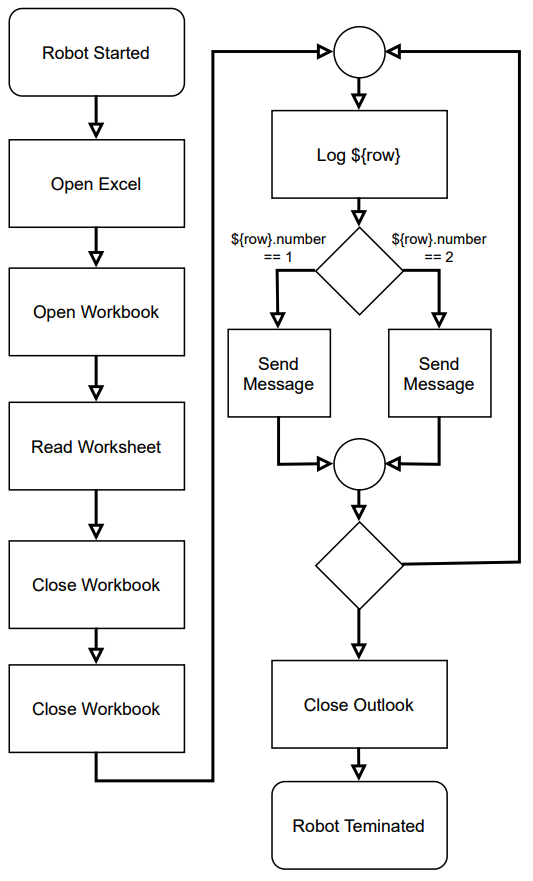
\includegraphics[width=0.5\textwidth]{Bachelorarbeit/images/ScreenshotFlowchart.png}
    \caption{Beispielprozess in Flowchart-Syntax}
    \label{fig:ScrFlow}
\end{figure}

Wie in der Abbildung \ref{fig:ScrFlow} zu sehen, eignen sich Flussdiagramme (engl. Flowchart) sehr gut für die Darstellung eines Softwareroboters. Der Arbeit ist eine Auflistung der elementaren logischen Ablaufstrukturen aus dem Werk von E. Hering \cite{Hering1984} beigefügt (Abbildung \ref{fig:UebersichtFlowchart}).

\subsubsection{Analyse der BPMN}
Wie in Abbildung \ref{fig:ScrBPMN} gezeigt, können sequenzielle Anweisungen in BPMN als Folge von Aktivitäten dargestellt werden. Verzweigungen lassen sich als XOR-Split mit entsprechenden Fallbedingungen abbilden. Ebenso können mit einem XOR-Split  Wiederholungen implementiert werden. Sofern Variablen auch in der visuellen Repräsentation sichtbar werden sollen, lassen sich diese durch Datenobjekte darstellen. 

\begin{figure}[h!]
    \centering
    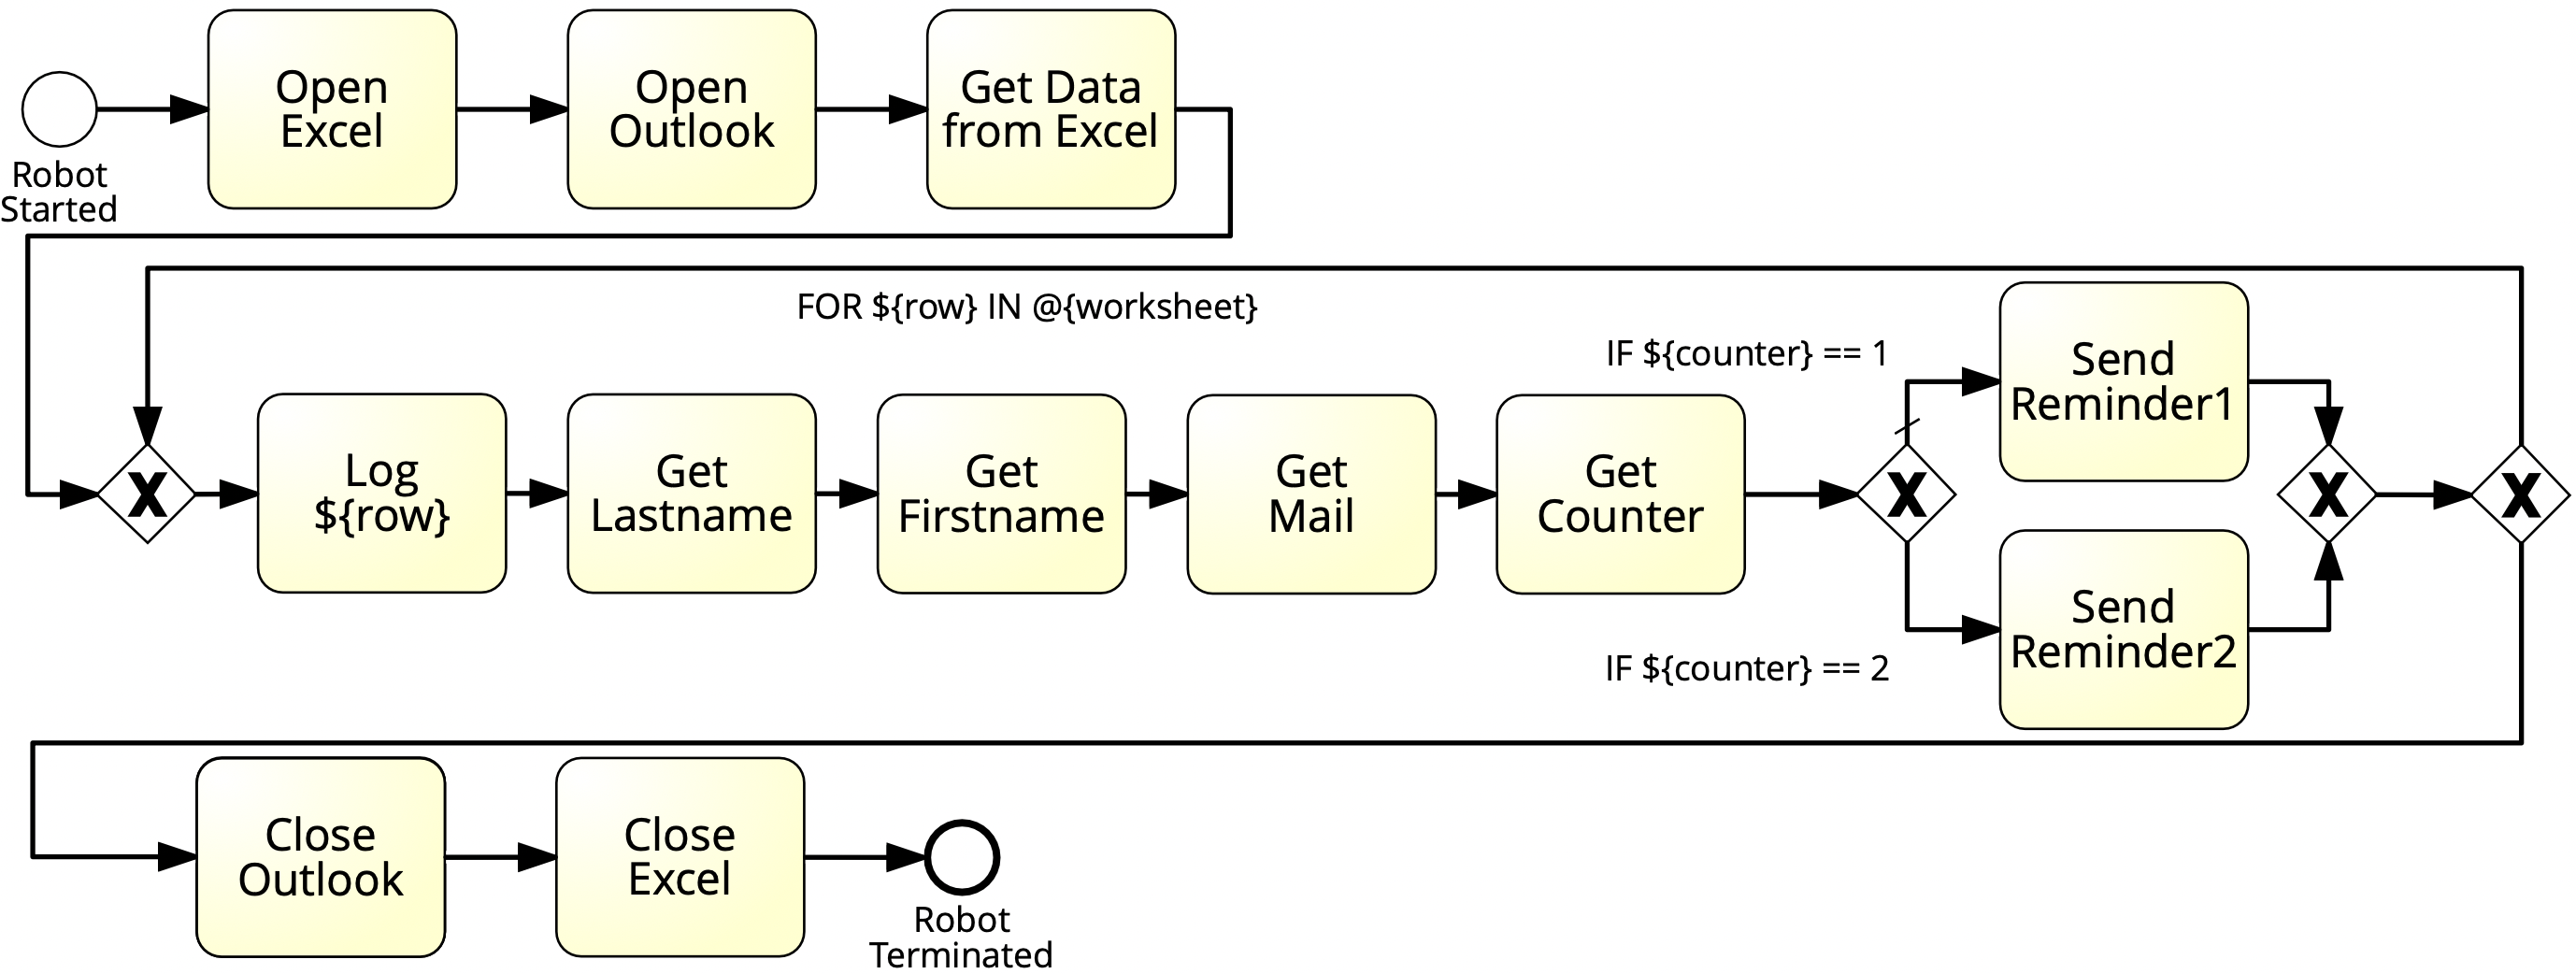
\includegraphics[width=1.0\textwidth]{Bachelorarbeit/images/ScreenshotBPMN4.png}
    \caption{Beispielprozess in BPMN-Syntax}
    \label{fig:ScrBPMN}
\end{figure}

Ursprünglich ist die Prozessmodellierungssprache BPMN nicht dafür konzipiert worden, Softwareabläufe darzustellen. Wie soeben gezeigt, eignet sich die Notation neben der Prozessmodellierung auch für die Implementierung von RPA-Robotern. Zudem bietet sie bereits im Standard die Möglichkeit alle Aktivitäten zu dokumentieren. Dieses Feature wurde von den RPA-Entwicklern ausdrücklich gewünscht und gilt als ein zentraler Vorteil der BPMN und des Programmablaufplans gegenüber anderen Prozessmodellierungssprachen.

\subsubsection{Analyse der EPK}

Die Ereignisgesteuerte Prozesskette wurde an der Universität des Saarlandes zusammen mit der SAP AG zur Dokumentation von Geschäftsprozessen entwickelt \cite{epkSyntax}.
Die EPK besitzt als Kernelemente das Ereignis, das einen Zustand im Prozess abbildet sowie die Funktion, die eine Aktion oder Aufgabe beschreibt. Jeder Prozess startet und endet mit einem Ereignis. Zwischen beiden Ereignissen können sequenzielle Anweisungen durch aneinandergereihte Funktionsaufrufe dargestellt werden. Durch Einsatz des XOR-Konnektors lassen sich analog zur BPMN (\mbox{Abbildung \ref{fig:ScrEPK}}) Verzweigungen sowie Schleifen darstellen.  Hierbei ist zu beachten, dass nach jeder XOR-Verzweigung zwingend ein Ereignis folgen muss, um den vorliegenden Zustand zu beschreiben. Diese Ereignis-Elemente dienen in unserem Fall zur Angabe der Fallbedingungen einer Verzweigung oder zur Darstellung der Schleifenabbruchbedingung.

\begin{figure}[h!]
    \centering
    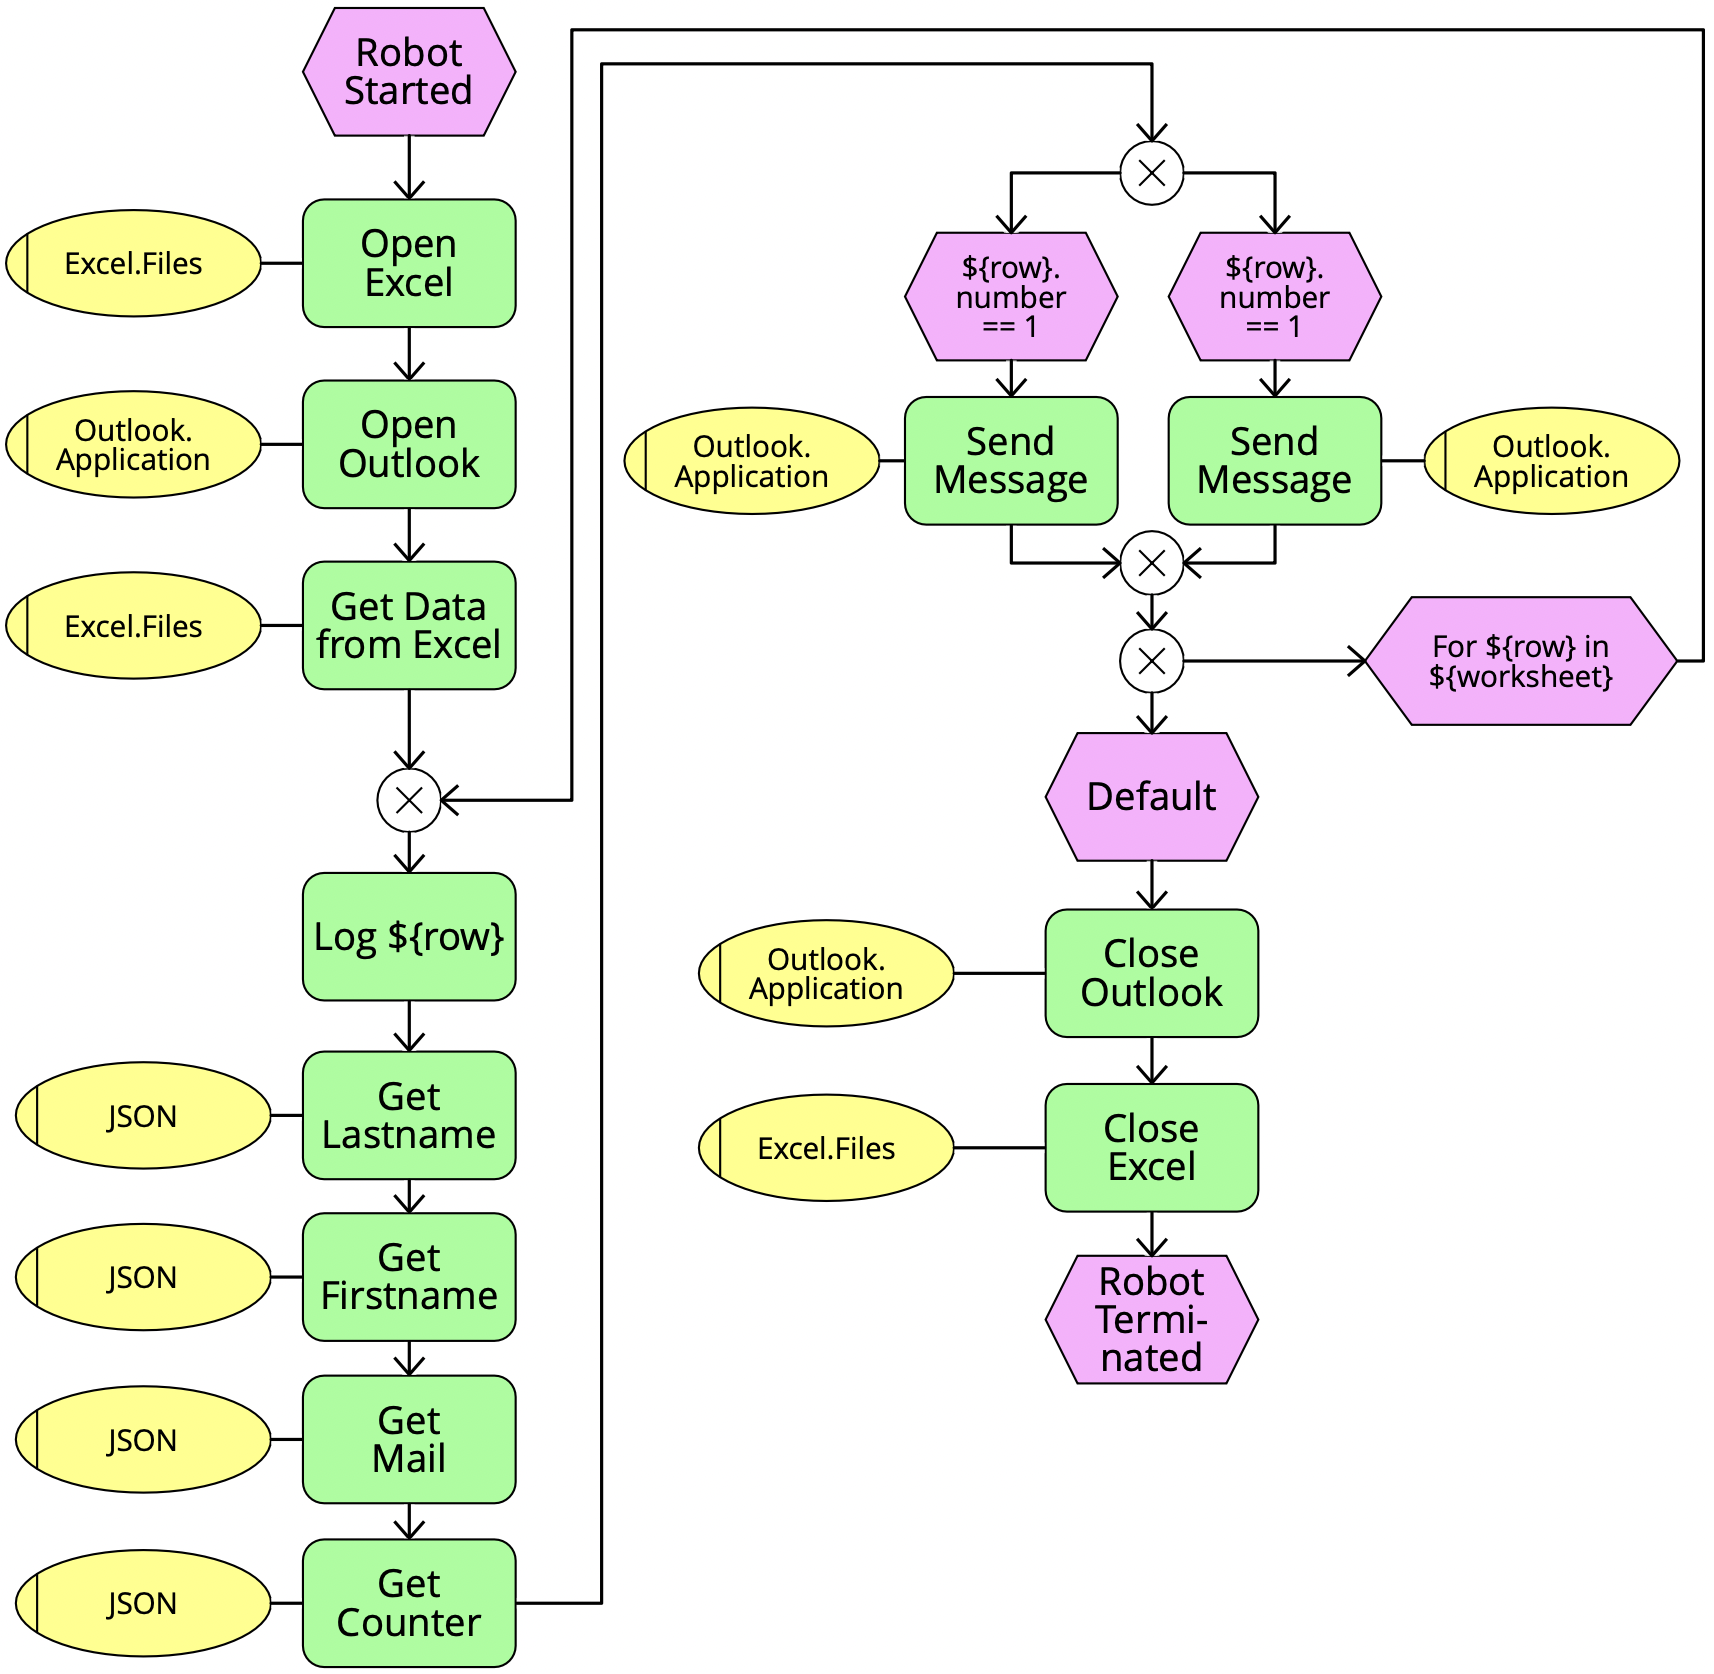
\includegraphics[width=0.75\textwidth]{Bachelorarbeit/images/ScreenshotEPK3.png}
    \caption{Beispielprozess in EPK-Syntax}
    \label{fig:ScrEPK}
\end{figure}

Wie beschrieben, lassen sich auch mit EPKs RPA-Roboter darstellen. Ähnlich zur BPMN können dem Diagramm Datenobjekte hinzugefügt und dadurch Variablen repräsentiert werden. Darüber hinaus lässt das „Organisationseinheit“-Element für die Darstellung der zum Ausführen der RPA-Aufgabe genutzten Anwendung (z.B. \code{Excel.Application}) verwenden. Dieses zusätzliche Element kann in der jedoch auch Visualisierung kann jedoch entfernt werden, da zu jeder Funktion die RPA-Anwendung gesondert im Seitenmenü spezifiziert werden muss.
	\clearpage
	
	\section{Erläuterung der einheitlichen Speicherlösung}\label{konzeption_ssot}

\tikzstyle{block} = [draw, fill=white!20, rectangle, 
    minimum height=3em, minimum width=6em]
\tikzstyle{sum} = [draw, fill=blue!20, circle, node distance=2cm]
\tikzstyle{input} = [coordinate]
\tikzstyle{output} = [coordinate]
\usetikzlibrary{arrows.meta,arrows}

Die Interviews des Kapitels \ref{anforderungsanalyse} ergaben, dass eine neue Plattform gewünscht wird, bei der das Wechseln zwischen verschiedenen visuellen Repräsentationen der Roboter möglich ist. Dadurch können sowohl Low-Code-Developer als auch professionelle Entwickler in ihrer präferierten Umgebung Automatisierungen erstellen.

Nachfolgend wird erläutert, mit welcher Architektur sich diese Funktionalität implementieren lässt und warum hierfür eine einheitliche Speicherlösung (Single Source of Truth) benötigt wird. Im Anschluss werden die Anforderungen an die SSoT dargestellt.

\subsection{Konzeption der Architektur}

Um die visuelle Repräsentation eines Roboters in den ausführbaren Code der RobotFramework Syntax zu übersetzen, werden die eingangs beschriebenen Parser benötigt. Sofern ausschließlich Robotermodelle in ausführbaren Code übersetzt werden sollen und somit kein Wechsel der Modellierungssprache bei der Erstellung eines Roboters möglich ist, genügt die in Abbildung \ref{fig:parser1} gezeigte Architektur. Hierbei wird für jeden Roboter die visuelle Repräsentation um die benötigten RPA-Eigenschaften angereichert und gespeichert. Im Beispiel von \code{bpmn-js} ist das Speicherformat ein XML, in dem jede BPMN-Aktivität um die Tags \code{<rpaApplication>} und \code{<rpaTask>} erweitert werden kann. Soll nun der Roboter ausgeführt werden, wird die aktuelle Version des XML-Files in den ausführbaren Code geparst. Dadurch wird für jedes unterstützte Interface genau ein Parser benötigt.

\begin{figure}[h!]
    \centering
    \begin{tikzpicture}[auto, show background rectangle, node distance=2cm,>=latex']
        \node [block, name= robot] (robot) {.ROBOT};
        \node [block, above left= 0.5cm and -0.5cm of robot, name=pap] {PAP};
        \node [block, above right= 0.5cm and -0.5cm of robot, name=epk] {EPK};
        \node [block, left=1cm of pap] (bpmn) {BPMN};
        \node [block, right=1cm of epk] (other) {...};
        \draw [-{Stealth[scale=2]}] (bpmn.south) -- (robot.west);
        \draw [-{Stealth[scale=2]}] (pap.south) -- (robot);
        \draw [-{Stealth[scale=2]}] (epk.south) -- (robot);
        \draw [-{Stealth[scale=2]}] (other.south) -- (robot.east);
    \end{tikzpicture}
    \caption{Lokation der Parser ohne Wechsel zwischen den Darstellungsformen}
    \label{fig:parser1}
\end{figure}

\clearpage

Um denselben Roboter in verschiedenen Notationen erstellen zu können, bedarf es in einer trivialen Lösung zwischen jedem Paar von Interfaces zweier Parser. Diese Variante der Implementierung ist in der Abbildung \ref{fig:parser2} dargestellt. Bei dieser und der nachfolgenden Lösung ist es zudem möglich, direkt in dem auszuführenden Code Änderungen vorzunehmen und diese im Anschluss auch in den Notationen zu sehen. Problematisch ist jedoch, dass bei dieser Architektur exponentiell viele Parser in Abhängigkeit der angebotenen Interfaces benötigt werden. Zudem müsste sich auf eine Repräsentation geeinigt werden, in der der Roboter persistent gespeichert wird. 

\begin{figure}[h!]
    \centering
    \begin{tikzpicture}[auto,show background rectangle, node distance=2cm,>=latex']
        \node [block, name= robot] (robot) {.ROBOT};
        \node [block, above left= 0.5cm and -0.5cm of robot, name=pap] {PAP};
        \node [block, above right= 0.5cm and -0.5cm of robot, name=epk] {EPK};
        \node [block, left=1cm of pap] (bpmn) {BPMN};
        \node [block, right=1cm of epk] (other) {...};
        \draw [{Stealth[scale=2]}-{Stealth[scale=2]}] (bpmn.south) -- (robot.west);
        \draw [{Stealth[scale=2]}-{Stealth[scale=2]}] (pap.south) -- (robot);
        \draw [{Stealth[scale=2]}-{Stealth[scale=2]}] (epk.south) -- (robot);
        \draw [{Stealth[scale=2]}-{Stealth[scale=2]}] (bpmn) -- (pap);
        \draw [{Stealth[scale=2]}-{Stealth[scale=2]}] (pap) -- (epk);
        \draw [{Stealth[scale=2]}-{Stealth[scale=2]}] (other.south) -- (robot.east);
        \draw [{Stealth[scale=2]}-{Stealth[scale=2]}] (other) -- (epk);
        \draw [{Stealth[scale=2]}-{Stealth[scale=2]}] (bpmn) to [out=25,in=155] (epk.north);
        \draw [{Stealth[scale=2]}-{Stealth[scale=2]}] (pap.north) to [out=25,in=155] (other);
        \draw [{Stealth[scale=2]}-{Stealth[scale=2]}] (bpmn.north) to [out=20,in=160] (other.north);
    \end{tikzpicture}
    \caption{Lokation der Parser ohne einheitliche Datenspeicherlösung}
    \label{fig:parser2}
\end{figure}

Um nur linear viele Parser zu benötigen, stellt diese Arbeit eine Architektur vor, die auf einer Single Source of Truth basiert. Diese SSoT dient als einheitliches Speicherformat der Roboter. Aus ihr werden alle visuellen Repräsentationen erstellt und ebenso resultieren alle Änderungen in den grafischen Editoren in der SSoT. Zur Realisierung dieses Konzeptes werden pro Notation zwei Parser benötigt (\mbox{Abbildung \ref{fig:parser3}).}

\begin{figure}[h!]
    \centering
    \begin{tikzpicture}[auto,show background rectangle, node distance=2cm,>=latex']
        \node [block, fill=black!30!green, rounded corners=0.5cm] (ssot) {SSoT};
        \node [block, above left= 0.7cm and 1.2cm of ssot, name=pap] {PAP};
        \node [block, above right= 0.7cm and 1.2cm of ssot, name=epk] {EPK};
        \node [block, left=2.65cm of ssot] (bpmn) {BPMN};
        \node [block, right=2.65cm of ssot] (other) {...};
        \node [block, above=0.7cm of ssot] (robot) {.ROBOT};
        \draw [{Stealth[scale=2]}-{Stealth[scale=2]}] (ssot) -- (robot);
        \draw [{Stealth[scale=2]}-{Stealth[scale=2]}] (ssot) -- (bpmn);
        \draw [{Stealth[scale=2]}-{Stealth[scale=2]}] (ssot) -- (epk.south);
        \draw [{Stealth[scale=2]}-{Stealth[scale=2]}] (ssot) -- (pap.south);
        \draw [{Stealth[scale=2]}-{Stealth[scale=2]}] (ssot) -- (other);
    \end{tikzpicture}
    \caption{Lokation der Parser mit einheitlicher Datenspeicherlösung}
    \label{fig:parser3}
\end{figure}

\clearpage

\subsection{Konzeption der Speicherlösung}

Betrachten wir nun das Konzept hinter der einheitlichen Speicherlösung. Diese Datenstruktur speichert alle relevanten Daten des Roboters, sodass daraus der finale Ausführungscode sowie alle visuellen Repräsentationen erstellt (engl. „geparst“) werden können.

Ziel der Speicherlösung ist es, die visuellen Repräsentationen zu abstrahieren und nur die Semantik zu speichern. Dafür wird für jede Modellierungssprache die ihr zugrunde liegende Programmierlogik abgeleitet und nur diese gespeichert. 
Für die Programmierkonzepte werden nachfolgend Typen definiert, mit deren Hilfe sich alle Graphen abspeichern lassen (siehe Tabelle \ref{tab:ssot-types}). Zusätzlich ist der Typ „\code{MARKER}“ definiert, der entweder Start oder Ende des Roboters beschreibt. Dadurch wird ermöglicht, die Start- und Endsymbole der BPMN, Flowcharts und EPKs - wie im Standard gewünscht - zu benennen. 

\begin{table}[h!]
    \caption{Typen der Single Source of Truth}
    \centering
        \begin{tabular}{|l|l|}
        \hline
        \textbf{Programming Construct} & \textbf{SSoT-Type} \\ \hline
        Single Statement               & INSTRUCTION       \\ \hline
        Branching                      & CASE              \\ \hline
        Loop                           & LOOP              \\ \hline
        Start / End of Robot           & MARKER            \\ \hline
        \end{tabular}
    \label{tab:ssot-types}
\end{table}

Die SSoT besteht aus einem Header, der die Meta-Informationen des Roboters wie die \code{RobotId}, den Namen des Roboters und die Id des ersten Knotens im Graphen speichert. Darauf folgt das \code{ElementArray}, das alle Programmteile des Roboters enthält.  Jedes Element des Element-Arrays besitzt ein Feld zur Angabe des Typs (\code{INSTRUCTION}, \code{CASE}, \code{LOOP} o. \code{MARKER}). Zudem wird für jedes Element der Name, eine Id, die Id der Vorgänger- und Nachfolger im Grahpen  sowie optional ein Dokumentationstext gespeichert. 

Wie in Abbildung \ref{fig:aufbauSSOT} zu sehen, kann jedes Element in Abhängigkeit des Typs um weitere Felder angereichert werden. Dazu zählen beispielsweise bei einer Anweisung (\code{INSTRUCTION}) die benötigten Informationen des RPA-Statements. Das Schleifen-Element (\code{LOOP}) speichert neben der Schleifenabbruchbedingung die Id’s der Anfangs- und Endknoten des Schleifenkörpers, um eine vollständige Rekonstruktion des Graphens zu ermöglichen. \code{MARKER} benötigen keine weiteren Attribute.

\begin{figure}[h!]
    \centering
    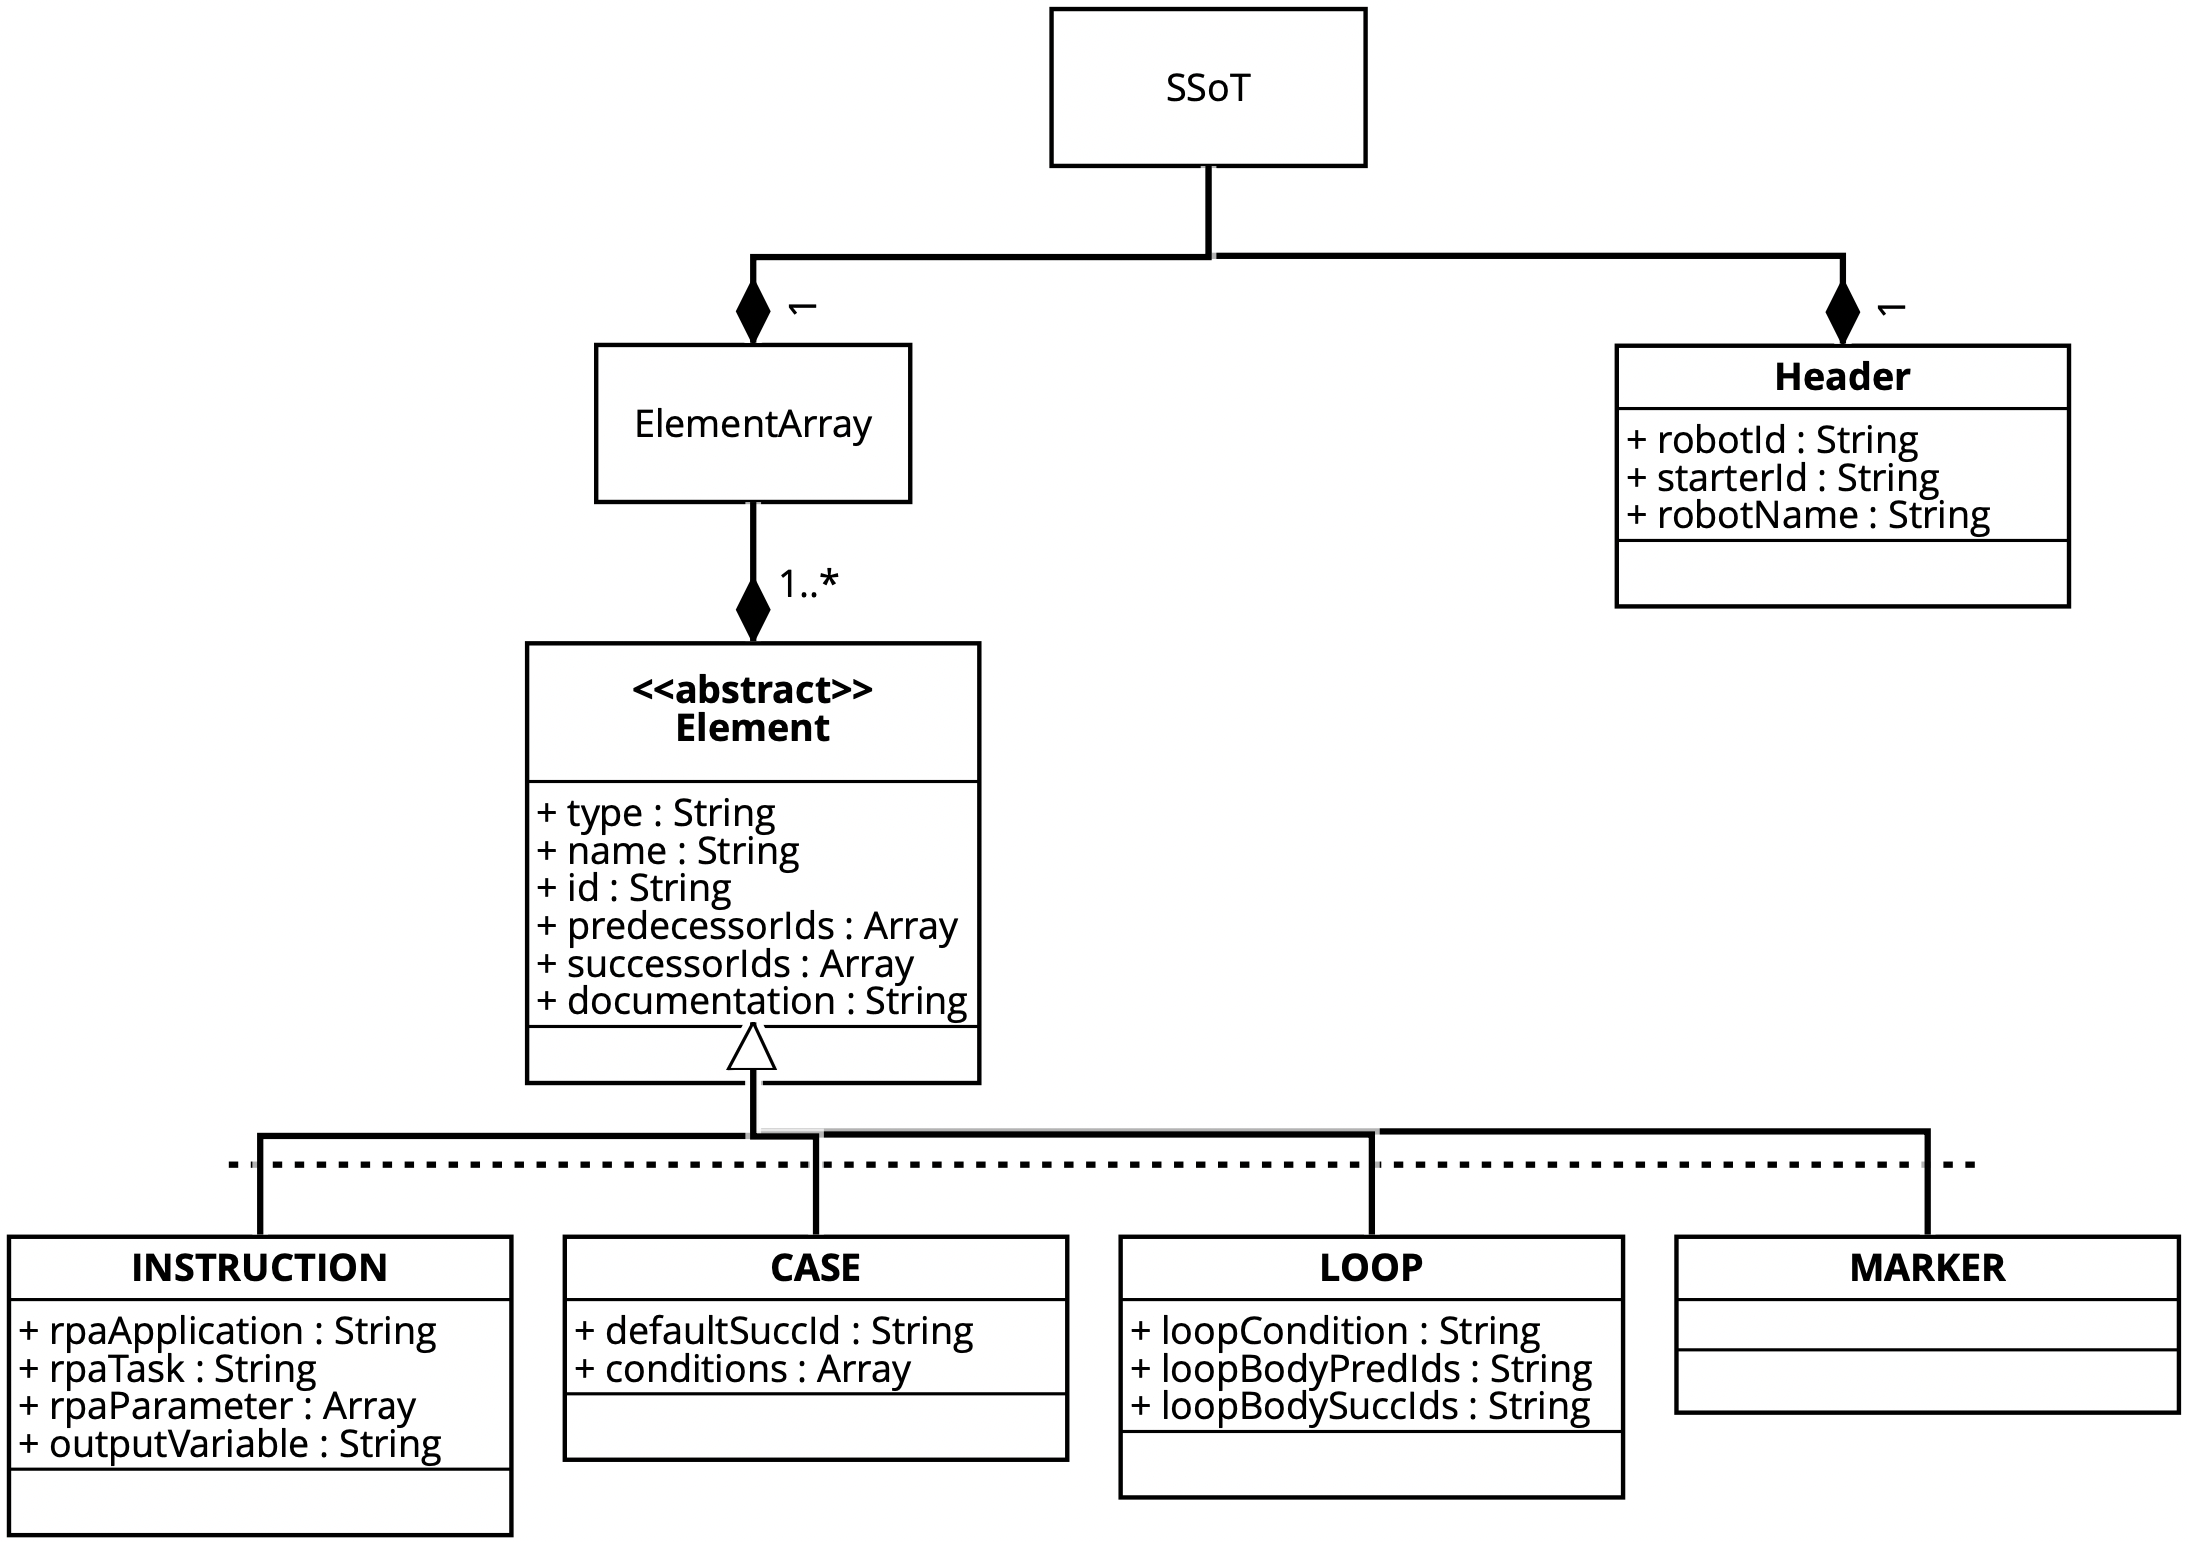
\includegraphics[width=1\textwidth]{Bachelorarbeit/images/aufbauSSOT2.png}
    \caption{Hierarchischer Aufbau der Datenspeicherlösung}
    \label{fig:aufbauSSOT}
\end{figure}

Der den Roboter beschreibende Graph lässt sich mit den Informationen zu Vorgänger- und Nachfolgerknoten eindeutig zusammensetzen. Somit kann aus der SSoT jede visuelle Repräsentation rekonstruiert werden. Es werden keine spezifischen Eigenschaften der Modellierungssprachen, wie zum Beispiel die absolute Position eines Knotens gespeichert. Daher müssen diese Werte auf Grundlage des Graphens errechnet werden, wodurch die Modelle sich bei jedem erneuten Rendering automatisch ausrichten und formatieren.

Die meisten Felder der Elemente werden mit Strings befüllt. Eine Besonderheit ist hierbei das \code{rpaParameter}-Array des \code{INSTRUCTION}-Elements. In diesem Array werden benötigte Eingabeparameter für die ausgewählte \code{rpaApplication/rpaTask}-Kombination angegeben. Somit kann dieses Array auch leer sein, sofern der Funktionsaufruf keine Parameter benötigt. 

\label{parameterProps}
Jeder Parameter repräsentiert wiederum ein Objekt, in dem der Name des Parameters, ein Hinweistext, eine boolesche Variable (die aussagt, ob der Parameter zwingend angegeben werden muss), sowie die Position des Parameters aus der RpaFramework-Dokumentation angegeben wird. Diese Ganzzahl gibt in Zusammenhang mit den anderen Parametern an, in welcher Ordnung die Parameter in den auszuführenden Code zu parsen sind.
Zudem werden für jeden Parameter der Typ wie beispielsweise \code{String} oder \code{Integer} sowie dessen Wert gespeichert.
	\clearpage
	
	\section{Implementierung der einheitlichen Speicherlösung}\label{implementierung_ssot}

Die nachfolgend beschriebene Implementierung ist als Proof of Concept im Open-Source-Projekt \code{ArkAutomate}\footnote{\url{https://github.com/bptlab/ark_automate} (Abgerufen am 22. Juni 2021)}  umgesetzt. Die Entwicklung erfolgte im Rahmen des der Abschlussarbeit zugrunde liegenden Projektes. Das Projektteam implementierte die in dieser Arbeit beschriebene einheitliche Datenspeicherlösung sowie die Modellierungsfunktion als ein Kernfeature der quelloffenen RPA-Plattform. Die SSoT ist in diesem Projekt als verschachteltes JavaScript Object implementiert. 

Betrachten wir nun das beidseitige Parsing zwischen der visuellen Repräsentation und der SSoT. Wie im vorangegangenen Kapitel beschrieben, werden zwischen jedem Interface und der SSoT zwei Parser benötigt. Ein Parser übersetzt das Modell in die SSoT und ein weiterer Parser erstellt aus der SSoT die visuelle Repräsentation.

Die Implementierung der Parser hängt stark von dem verwendeten Modellierungsmodul ab. Das im Proof of Concept verwendete npm-Paket \code{bpmn-js}\footnote{\url{https://www.npmjs.com/package/bpmn-js} (Abgerufen am 22. Juni 2021} zeichnete sich durch seine umfangreichen Funktionen und Anpassungsmöglichkeiten des Modelers aus. Zur Modellierung von Flowcharts bietet sich eine Erweiterung des \code{react-flow-diagram} Paketes\footnote{\url{https://www.npmjs.com/package/react-flow-diagram} (Abgerufen am 22. Juni 2021)} an. Es lässt sich um die unterstützten Sinnbilder erweitern. Einen Modeler-Package zur Erstellung von Ereignisgesteuerten Prozessketten konnte nicht gefunden werden. Dies kann an der geringen Verbreitung der Notation außerhalb des deutschsprachigen Raumes liegen.

Nachfolgend werden die grundlegenden Konzepte der Parser an den im Proof of Concept verwendeten Notationen BPMN und dem finalen Ausführungscode beschrieben.

\subsection{Übersetzung der SSoT in eine visuelle Repräsentation}

Betrachten wir zuerst den Parser, der den RobotFramework Code erzeugt. Zu Beginn dieses Codes müssen die verwendeten RpaFramework Librarys aufgeführt werden (Abbildung \ref{fig:ScrRobotFr}). Hierfür genügt eine Iteration über das \code{ElementArray}, bei der alle verwendeten Applikationen gespeichert werden. Der Graph lässt sich mit einer rekursiven Betrachtung des \code{ElementArray}s rekonstruieren, wodurch der RobotFramework Code zeilenweise wächst. 

Komplizierter hingegen ist die Erstellung von Modellen aus der SSoT. Hierbei sind die verwendeten XMLs oft sehr komplex und erfordern eine Vielzahl an Parametern wie Positionen der Elemente und Verbindungen. Für das Paket \code{bpmn-js} existiert jedoch ein Command Line Interface (CLI)\footnote{\url{https://www.npmjs.com/package/bpmn-js-cli} (Abgerufen am 22. Juni 2021)}, das die Ausrichtung der BPMN-Komponenten übernimmt. So genügt es, dem BPMN-Diagramm die Elemente in der sortierten Reihenfolge mittels \code{cli.append(element)} hinzuzufügen. Das anzuzeigende XML mit allen Positionswerten wird durch das Interface erstellt.  

\subsection{Übersetzung einer visuellen Repräsentation in die SSoT}

Zur einfacheren Speicherung der Informationen eines Roboters wird in der Implementierung der eigentliche Graph getrennt von den Eigenschaften jedes Knotens gespeichert. Die Informationen zu \code{rpaApplication} und \code{rpaTask} werden zusammen mit einer Referenz auf das betreffende \code{INSTRUCTION}-Element in der \code{localAttributeStorage} abgelegt. In diesem einen Objekt der Session Storage werden somit direkt alle Änderungen an der \mbox{RPA Task / Application-Kombination} vermerkt. Das \code{localParameterStorage}-Objekt speichert zu jedem \code{INSTRUCTION}-Element ein Array aller Parameter mit den in Abbildung \ref{fig:aufbauSSOT} vorgestellten Feldern. Die Seitenleiste (\code{ModelerSidebar}) bietet die Möglichkeit, alle Parameter eines Elements zu verändern. Die Änderungen werden direkt in den betreffenden Objekten der Session Storage geändert. Die \code{ModelerSidebar} ist modular aufgebaut und kann daher weiteren in Modellierungsinterfaces wiederverwendet werden.

Betrachten wir nun das Parsing - die eigentliche Erstellung der SSoT. Hierbei lassen sich für alle Parser dieser Richtung einige Gemeinsamkeiten festhalten. Jeder Parser erstellt zuerst den SSoT-Header mit den beschriebenen drei Feldern. Im Anschluss muss das \code{ElementArray} erstellt werden, sodass dann beide Teile zur SSoT zusammengefügt und gespeichert werden können. 

Sofern die Daten in einer nicht strukturierten Form vorliegen, müssen sie vorab aufbereitet werden. Dieser Schritt geschieht beim RobotFramework Code durch zeilenweises Einlesen. Die Daten des \code{bpmn-js} liegen im XML-Format vor und müssen daher ebenso vorab bearbeitet werden. Das XML lässt sich in der JavaScript Anwendung schwer verarbeiten, weshalb es in der Projektarbeit mit dem \code{xmljs2}-Paket\footnote{\url{https://www.npmjs.com/package/xmljs2} (Abgerufen am 22. Juni 2021)} in ein JavaScript Objekt gewandelt wurde. Auf dieser Grundlage können die Elemente durch eine einfache Iteration über die strukturierten Daten erstellt werden. Der BPMN-Parser muss das \code{bpmn-js}-XML um die Informationen der ausgelagerten Objekte aus der Session Storage anreichern.  

\subsection{Evaluation der Lösung}
\label{evaluation_ssot}

Die vorgestellte Lösung, die in ersten Teilen im Proof of Concept implementiert wurde, ermöglicht das Bearbeiten der Roboter in verschiedenen Modellierungssprachen. Die Parser, die aus der SSoT die visuelle Repräsentation des Roboters erstellen, ließen sich leicht implementieren. Das lag vor allem an dem durch Camunda bereitgestellten Interface sowie dem \code{bpmn-js} Modeler. Sofern diese Tools für eine Modellierungssprache - wie beispielsweise die EPKs - nicht zur Verfügung stehen, erhöht sich der Arbeitsaufwand zur Anbindung weiterer Interfaces erheblich. Aufwändig ist vor allem das korrekte Ausrichten der Elemente des Modells, was im Beispiel des BPMN-Editors das CLI übernahm.

Die Parser, die beim Speichern den Roboter in die SSoT übersetzen, implementieren sich vergleichsweise komplizierter. Um Fehler bei der Erstellung der SSoT zu vermeiden, ist eine komplexe Fehlerbehandlung notwendig, die unsaubere Eingaben des Codes abfängt. Gleiches gilt für den Parser, der das BPMN-Diagramm in die SSoT übersetzt. Sobald ein Fehler beim Übersetzen festgestellt wird, bricht der Parser ab und es wird keine SSoT an den Server gesendet. Bei beiden Parsern wird ein besonderer Fokus auf aussagekräftige Fehlermeldungen gelegt, die den Nutzern bei der Bedienung helfen. So wird der Entwickelnde unter anderem gewarnt, wenn das BPMN-Modell zwei Start-Ereignisse besitzt (Abbildung \ref{fig:errorBPMN}) oder wenn ein Schreibfehler im Code-Editor erkannt wird (Abbildung \ref{fig:errorROBOT}).

\begin{figure}[!htb]
    \centering
    \begin{minipage}{.5\textwidth}
        \centering
        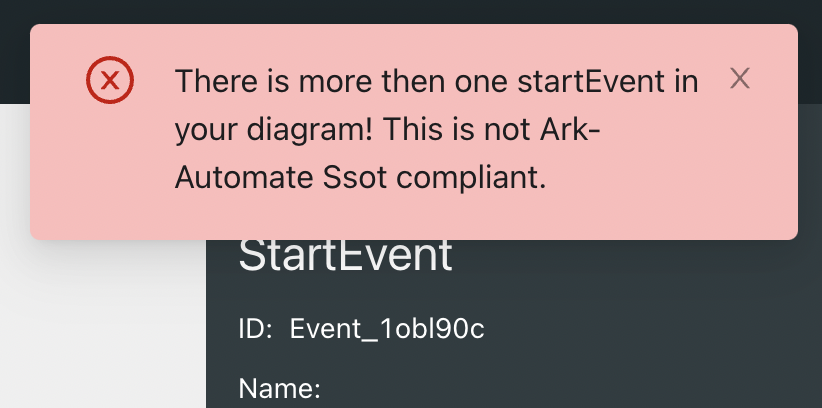
\includegraphics[width=0.95\textwidth, height=0.17\textheight]{Bachelorarbeit/images/ScreenshotErrorBPMN3.png}
        \caption{Fehlermeldung \\ BPMN-Editor}
        \label{fig:errorBPMN}
    \end{minipage}%
    \begin{minipage}{0.5\textwidth}
        \centering
        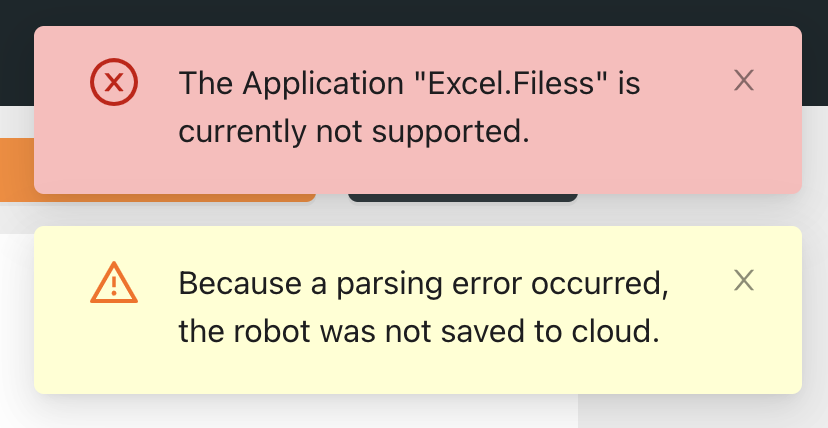
\includegraphics[width=0.95\textwidth, height=0.17\textheight]{Bachelorarbeit/images/ScreenshotErrorROBOT.png}
        \caption{Fehlermeldung \\ Code-Editor}
        \label{fig:errorROBOT}
    \end{minipage}
\end{figure}

Das Proof of Concept unterstützt aktuell die Element-Typen \code{MARKER} und \code{INSTRUCTION}. Um weitere Typen zu unterstützen, ist eine Umstellung des \mbox{RobotFramework} Codes auf die Keywords-Syntax notwendig. Hierfür müssen die zwei betreffenden Parser angepasst werden. Die Keywords-Syntax ermöglicht das Zusammenfassen von Programmteilen ähnlich der Definition von Funktionen in der objektorientierten Programmierung. Diese Funktionen werden als Keywords bezeichnet und im Hauptprogramm semantisch aneinandergereiht (Abbildung \ref{fig:ScrRobotFrKeywords}). Sobald diese Umstellung erfolgt, lassen sich auch die beschriebenen Konzepte der Schleife und der Verzweigung implementieren. Mit der Weitentwicklung der Plattform ließe es sich zudem implementieren, einzelne Programmbausteine mehrfach zu verwenden.

Aus meiner persönlichen Erfahrung heraus ist die Bedienung des RobotFramework Editors sehr umständlich. Prinzipiell lassen sich im Code-Editor Automatisierungen mit weniger Klicks implementieren als im BPMN-Editor, jedoch fehlen vor allem eine Auto-Vervollständigung sowie eine Schnellvorschau beim Schreiben des Codes. Aktuell existiert keine Möglichkeit, die Aktivitäten einer Library sowie  die benötigten Parameter angezeigt zu bekommen. Daher ist das Programmieren momentan nur für Experten, die alle zu verwendenden Befehle kennen, möglich. In Zukunft kann die Weiterentwicklung des Robot Framework Language Servers\footnote{\url{https://marketplace.visualstudio.com/items?itemName=robocorp.robotframework-lsp} \\ (Aufgerufen am 24.07.2021)} eingebunden werden, die eine Code-Vervollständigung sowie Syntax-Validierung unterstützt.

Aus meiner Sicht bietet es sich an, für erfahrenere Entwickler, die keine Erfahrung in der Modellierung haben, ein Low-Code-Interface wie Google Blockly\footnote{\url{https://developers.google.com/blockly} (Abgerufen am 12.07.2021)} bereitzustellen. Google Blockly ermöglicht die Programmierung in einem grafischen Code-Editor durch die Aneinanderreihung von Funktionsblöcken. Blockly ist unter anderem die dem grafischen Code-Editor zugrunde liegende Library des  MIT AppInventors. 


	\clearpage
	
	\section{Zusammenfassung und Ausblick}
\label{conclusion}

In den eingangs dokumentierten Interviews wurde festgestellt, dass aktuell die Erstellung und Dokumentation von RPA-Robotern in verschiedenen Programmen erfolgen muss. Mit der vorgestellten Lösung ist es möglich, RPA-Roboter direkt in BPMN zu modellieren und die Automatisierungsfolgen zu implementieren. Zudem ist es durch die SSoT erstmals möglich, denselben Roboter in verschiedenen Modellierungsnotationen und Code-Editoren zu erstellen. Die einheitliche Speicherlösung und das Konzept der Parser ermöglichen darüber hinaus, weitere Modellierungsinterfaces, aber auch Code-Editoren zu ergänzen. Die Anbindung von Modellierungsinterfaces sowie zukünftig einem Low-Code-Editor, wie beipielsweise Google Blockly, ermöglicht auch für Prozessexperten ohne IT-Hintergrund die Erstellung von RPA-Robotern. Ebenso kann ein Entwickler den Roboter direkt im Code erstellen und trotzdem die für Prozessexperten relevante Dokumentation in Form eines BPMN-Diagramms bereitstellen. Sofern gewünscht, könnten Prozessexperten kleinere Änderungen an der Automatisierung in einem für sie geeigneteren Interface direkt vornehmen.

RPA-Automatisierungen sollten aus meiner Sicht in jedem Fall von RPA-Consultants begleitet werden. Andernfalls wird der Schritt der Prozessoptimierung (zum Beispiel mit Process Mining) oftmals vernachlässigt. Auch in den Interviews mit den RPA-Entwicklern wurde deutlich, dass vor jeder Automatisierung mögliches Optimierungspotenzial analysiert wird.

Die aktuelle Implementierung, die für jede Aktivität einen einzelnen Test-Case definiert, unterstützt keine lokalen Variablen, Verzweigungen und Schleifen. Um diese Konstrukte abbilden zu können, muss der RobotFramework-Code auf die Keywords-Syntax umgestellt werden. Wie der Code für unserem Beispielprozess in dieser Syntax strukturiert ist, zeigt der Code-Ausschnitt in Abbildung \ref{fig:ScrRobotFrKeywords}. Die dort vorgestellte Syntax ermöglicht langfristig die Umsetzung aller in dieser Arbeit vorgestellten Konzepte. Durch die Trennung der RPA-Funktionen und der Programmstruktur ist der Code zudem besser lesbar. 
Sofern eine Umstellung auf die Keywords-Syntax erfolgt, ist zu prüfen, ob alle verwendeten Algorithmen zur Rekonstruktion des Graphenmodells korrekt funktionieren. Die bestehenden Tests decken nur sequenzielle Folgen von Anweisungen ab.

\clearpage

Eine durch die SSoT entstehende Einschränkung ist die Abstraktion der Modelle. So kann BPMN in der Standarddefinition deutlich mehr abbilden, als sich aufgrund des SSoT-Modells speichern lässt. Viele Details lassen sich nicht in den Code überführen oder in anderen Modellierungssprachen darstellen. Alle Eigenschaften, die sich nicht auf andere Modellierungsnotationen übertragen lassen, werden nicht in der SSoT gespeichert und stehen daher auch nicht in BPMN zur Verfügung.
Dazu zählen unter anderem wesentliche Dokumentationsfeatures, aber auch Konzepte wie beispielsweise Pools, Lanes und aufklappbare Subprozesse. Letztere können, wie in Abbildung \ref{fig:viadee} erkenntlich, die Übersichtlichkeit der Prozessdarstellung erheblich verbessern. Zudem lassen sich über diese Syntax wiederverwendbare, modulare Roboter abbilden. Diese Funktion passt zur Anforderung von UiPath \cite{uiPathReq}, eine Integrationsmöglichkeit für Roboter aus der \glqq globalen Anwender-Community\grqq{} anzubieten.

Ein möglicher Nachteil der SSoT-Lösung und der damit einhergehenden Nicht-Speicherung von interfacespezifischen Daten ist die automatische Ausrichtung aller Diagrammelemente bei jeder Öffnung des Modelers. Alle Elemente der visuellen Repräsentation - in BPMN - werden jedes Mal neu positioniert. Das kann einerseits gewollt sein, da zum Beispiel das \code{bpmn-js} CLI versucht, alle Elemente strukturiert anzuordnen. Andererseits wird keine manuell gewünschte Änderung in der Anordnung der Elemente gespeichert, wie sie beispielsweise zur besseren Übersicht beim Drucken des Diagramms gewünscht sein kann. Dieses Feature kann sich nur dann umgesetzt werden, wenn die in der Abbildung \ref{fig:parser1} dargestellte Architektur verwendet wird. Dann lässt sich jeder Roboter nur in genau einem Modellierungsinterface erstellen und zu jeder Ausführung in den RobotFramework Code parsen. Da ein Entwicklerteam mit genau einer Modellierungssprache arbeitet, kann sich diese Einschränkung auszahlen.  

Abschließend ist festzuhalten, dass der Wunsch der RPA-Developer nach einer Plattform, die das Erstellen von Robotern mit verschiedenen Modellierungssprachen ermöglicht, erfüllt werden konnte. Hierzu wurde eingehend untersucht, welche Modellierungssprachen sich für die Erstellung der Roboter eignen. Durch die Proof of Concept Implementierung wurde das Konzept der einheitlichen Speicherlösung validiert. Mit der entstandenen Implementierung wurde eine Open-Source-RPA-Plattform geschaffen, die sich um weitere benötigte Interfaces erweitern lässt.

	% bibliography
	\cleardoublepage
	%\bibliographystyle{plain}
	%\bibliographystyle{abbrvdin}
	\bibliographystyle{alphadin}
	\bibliography{bibliography/references}
	\cleardoublepage
	
	\appendix
\section{Anhang}

\begin{figure}[h!]
    \centering
    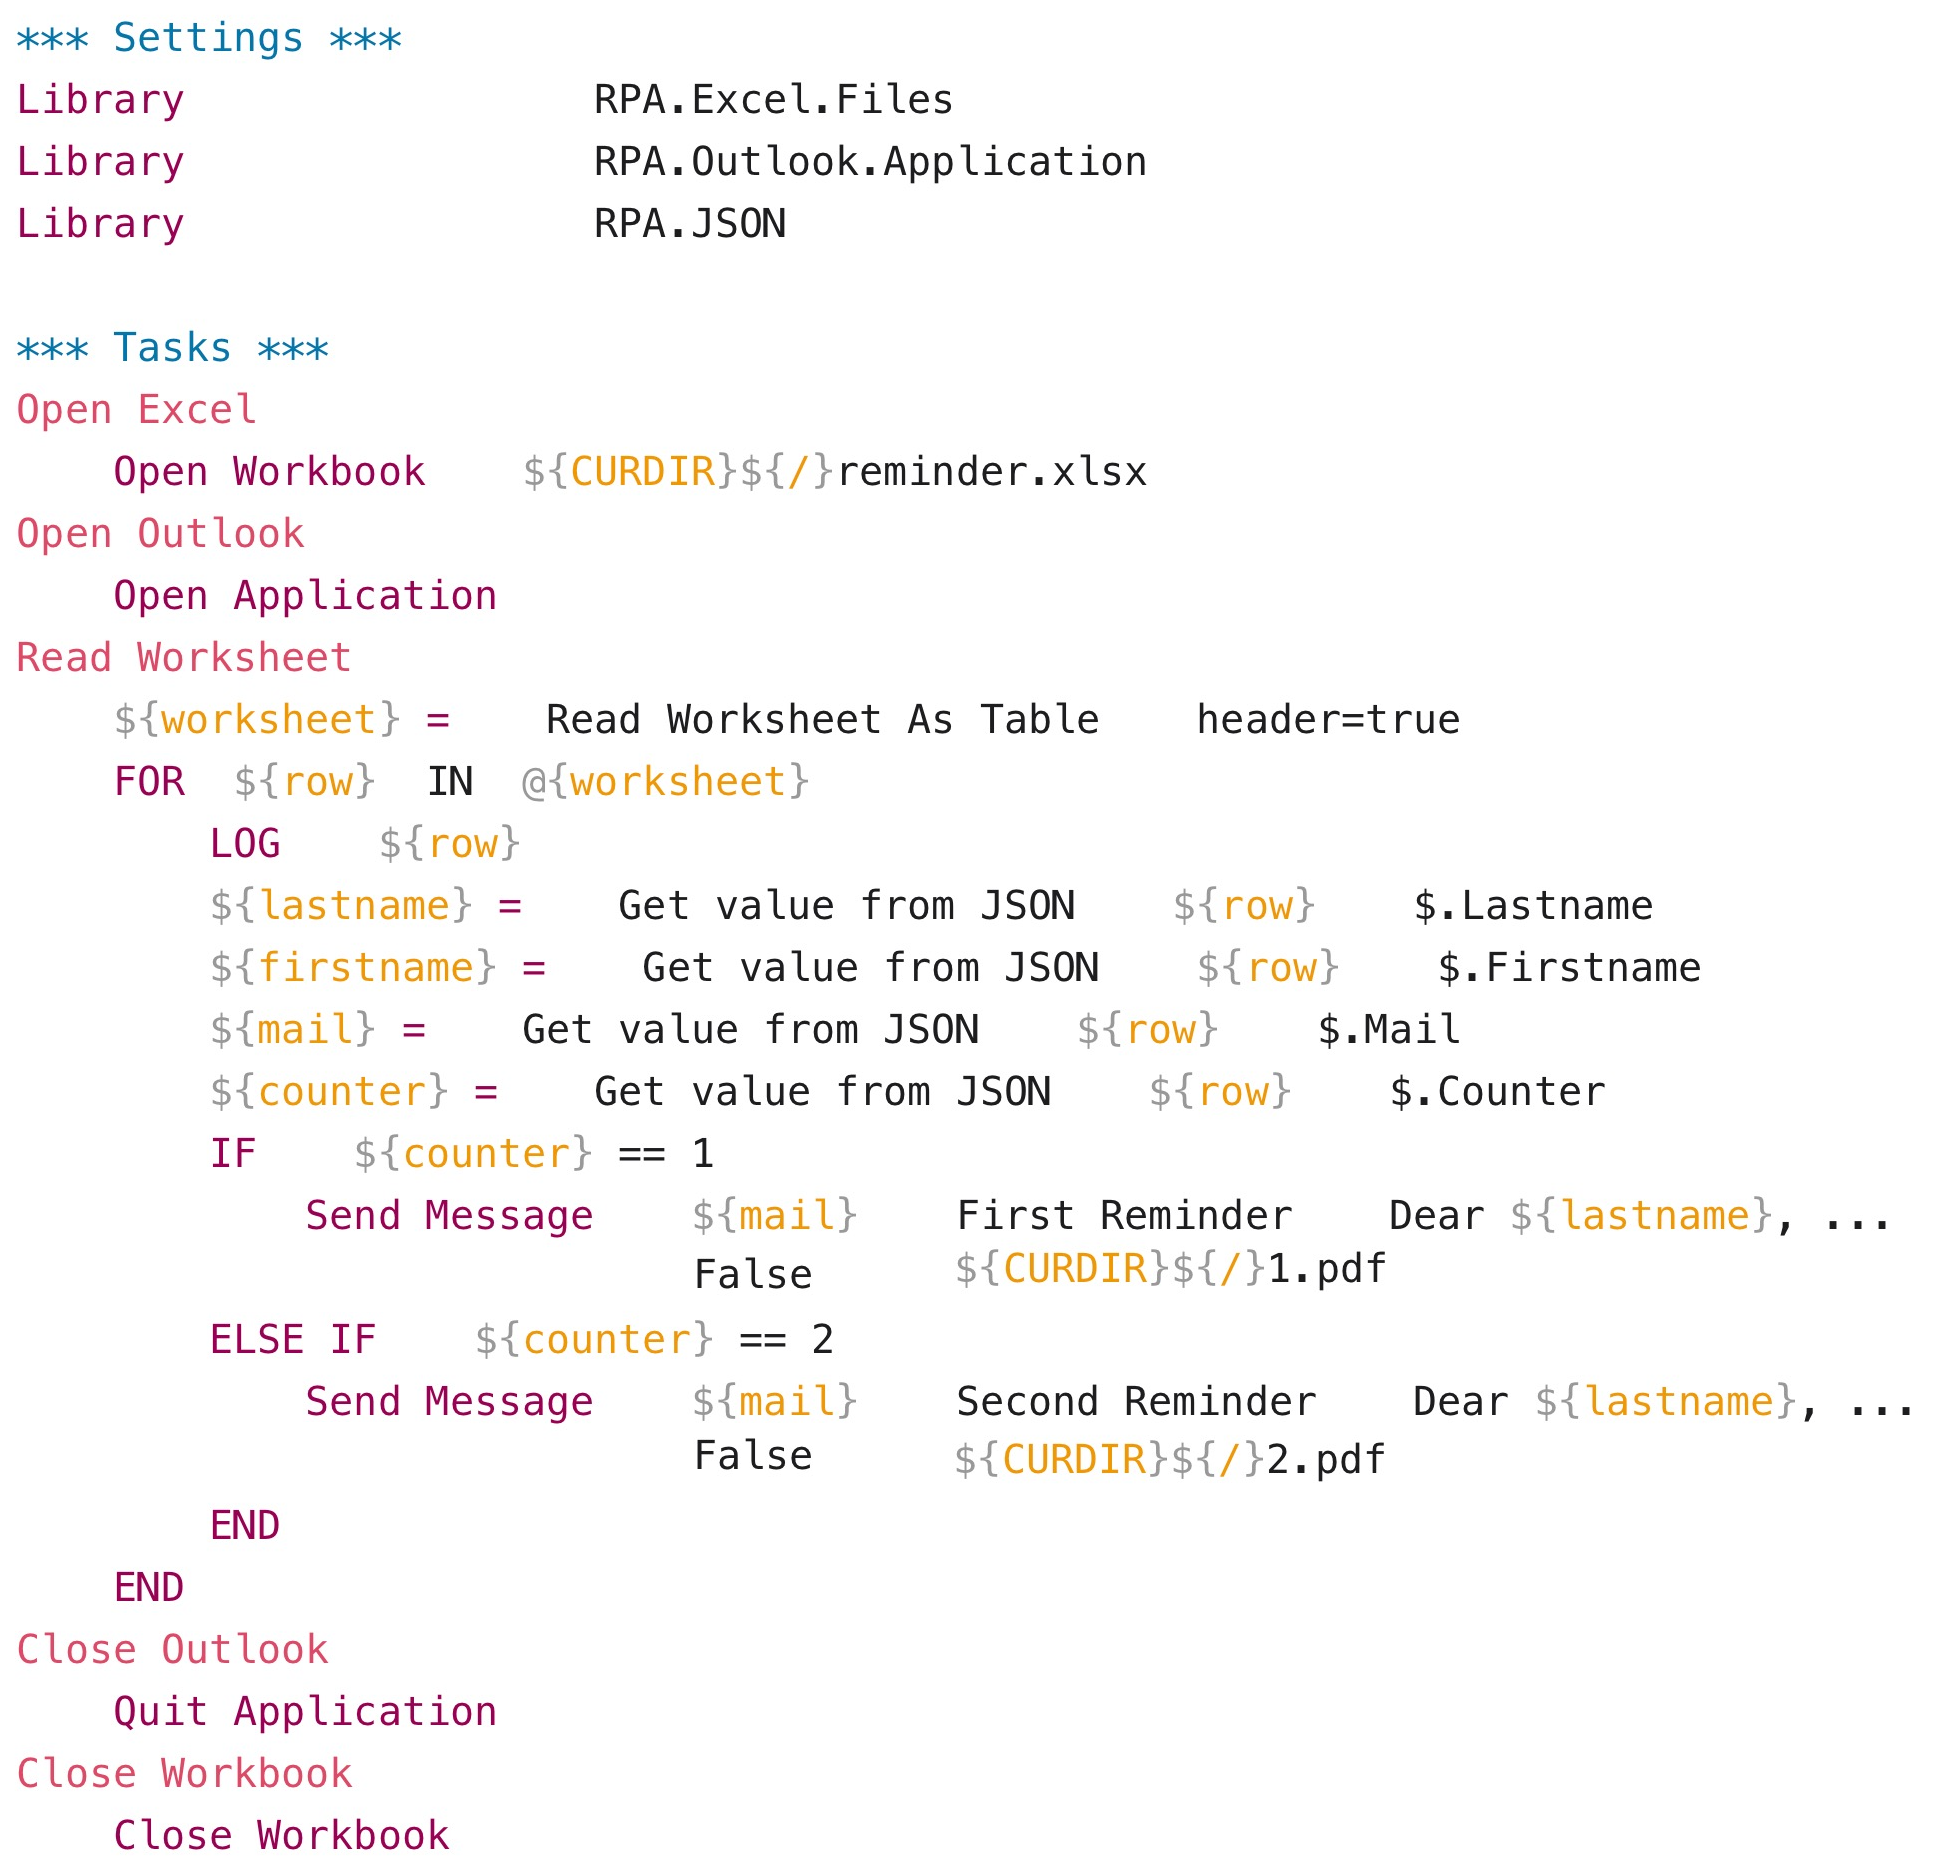
\includegraphics[width=1.0\textwidth]{Bachelorarbeit/images/exampleBot2_v4.png}
    \caption{Beispielprozess in RobotFramework-Syntax}
    \label{fig:ScrRobotFr}
\end{figure}

\begin{figure}[h!]
    \centering
    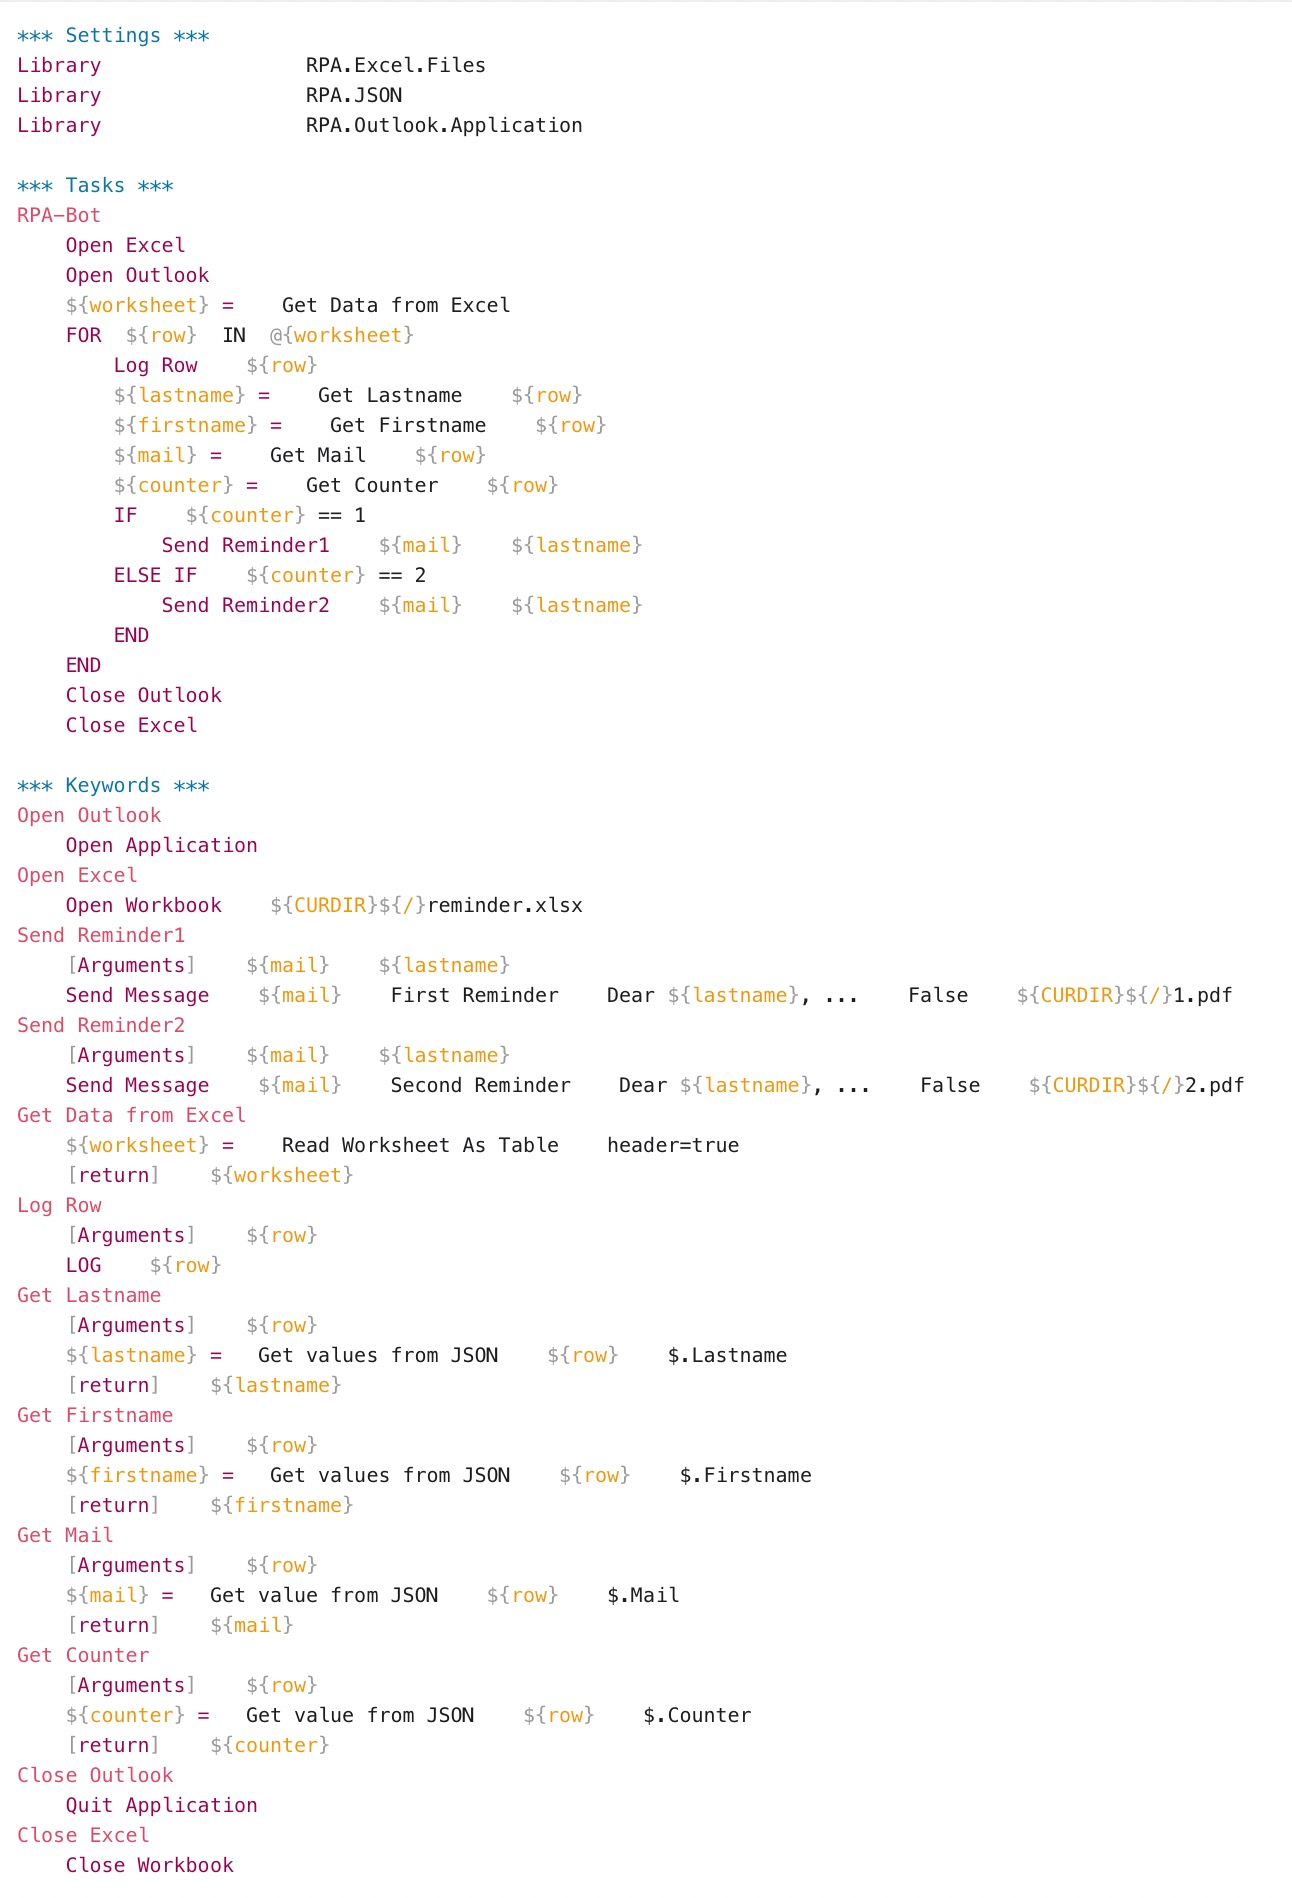
\includegraphics[width=0.95\textwidth]{Bachelorarbeit/images/exampleBotKeywords2.png}
    \caption{Beispielprozess in RobotFramework-Syntax unter Verwendung der Keywords}
    \label{fig:ScrRobotFrKeywords}
\end{figure}

\begin{figure}[h!]
    \centering
    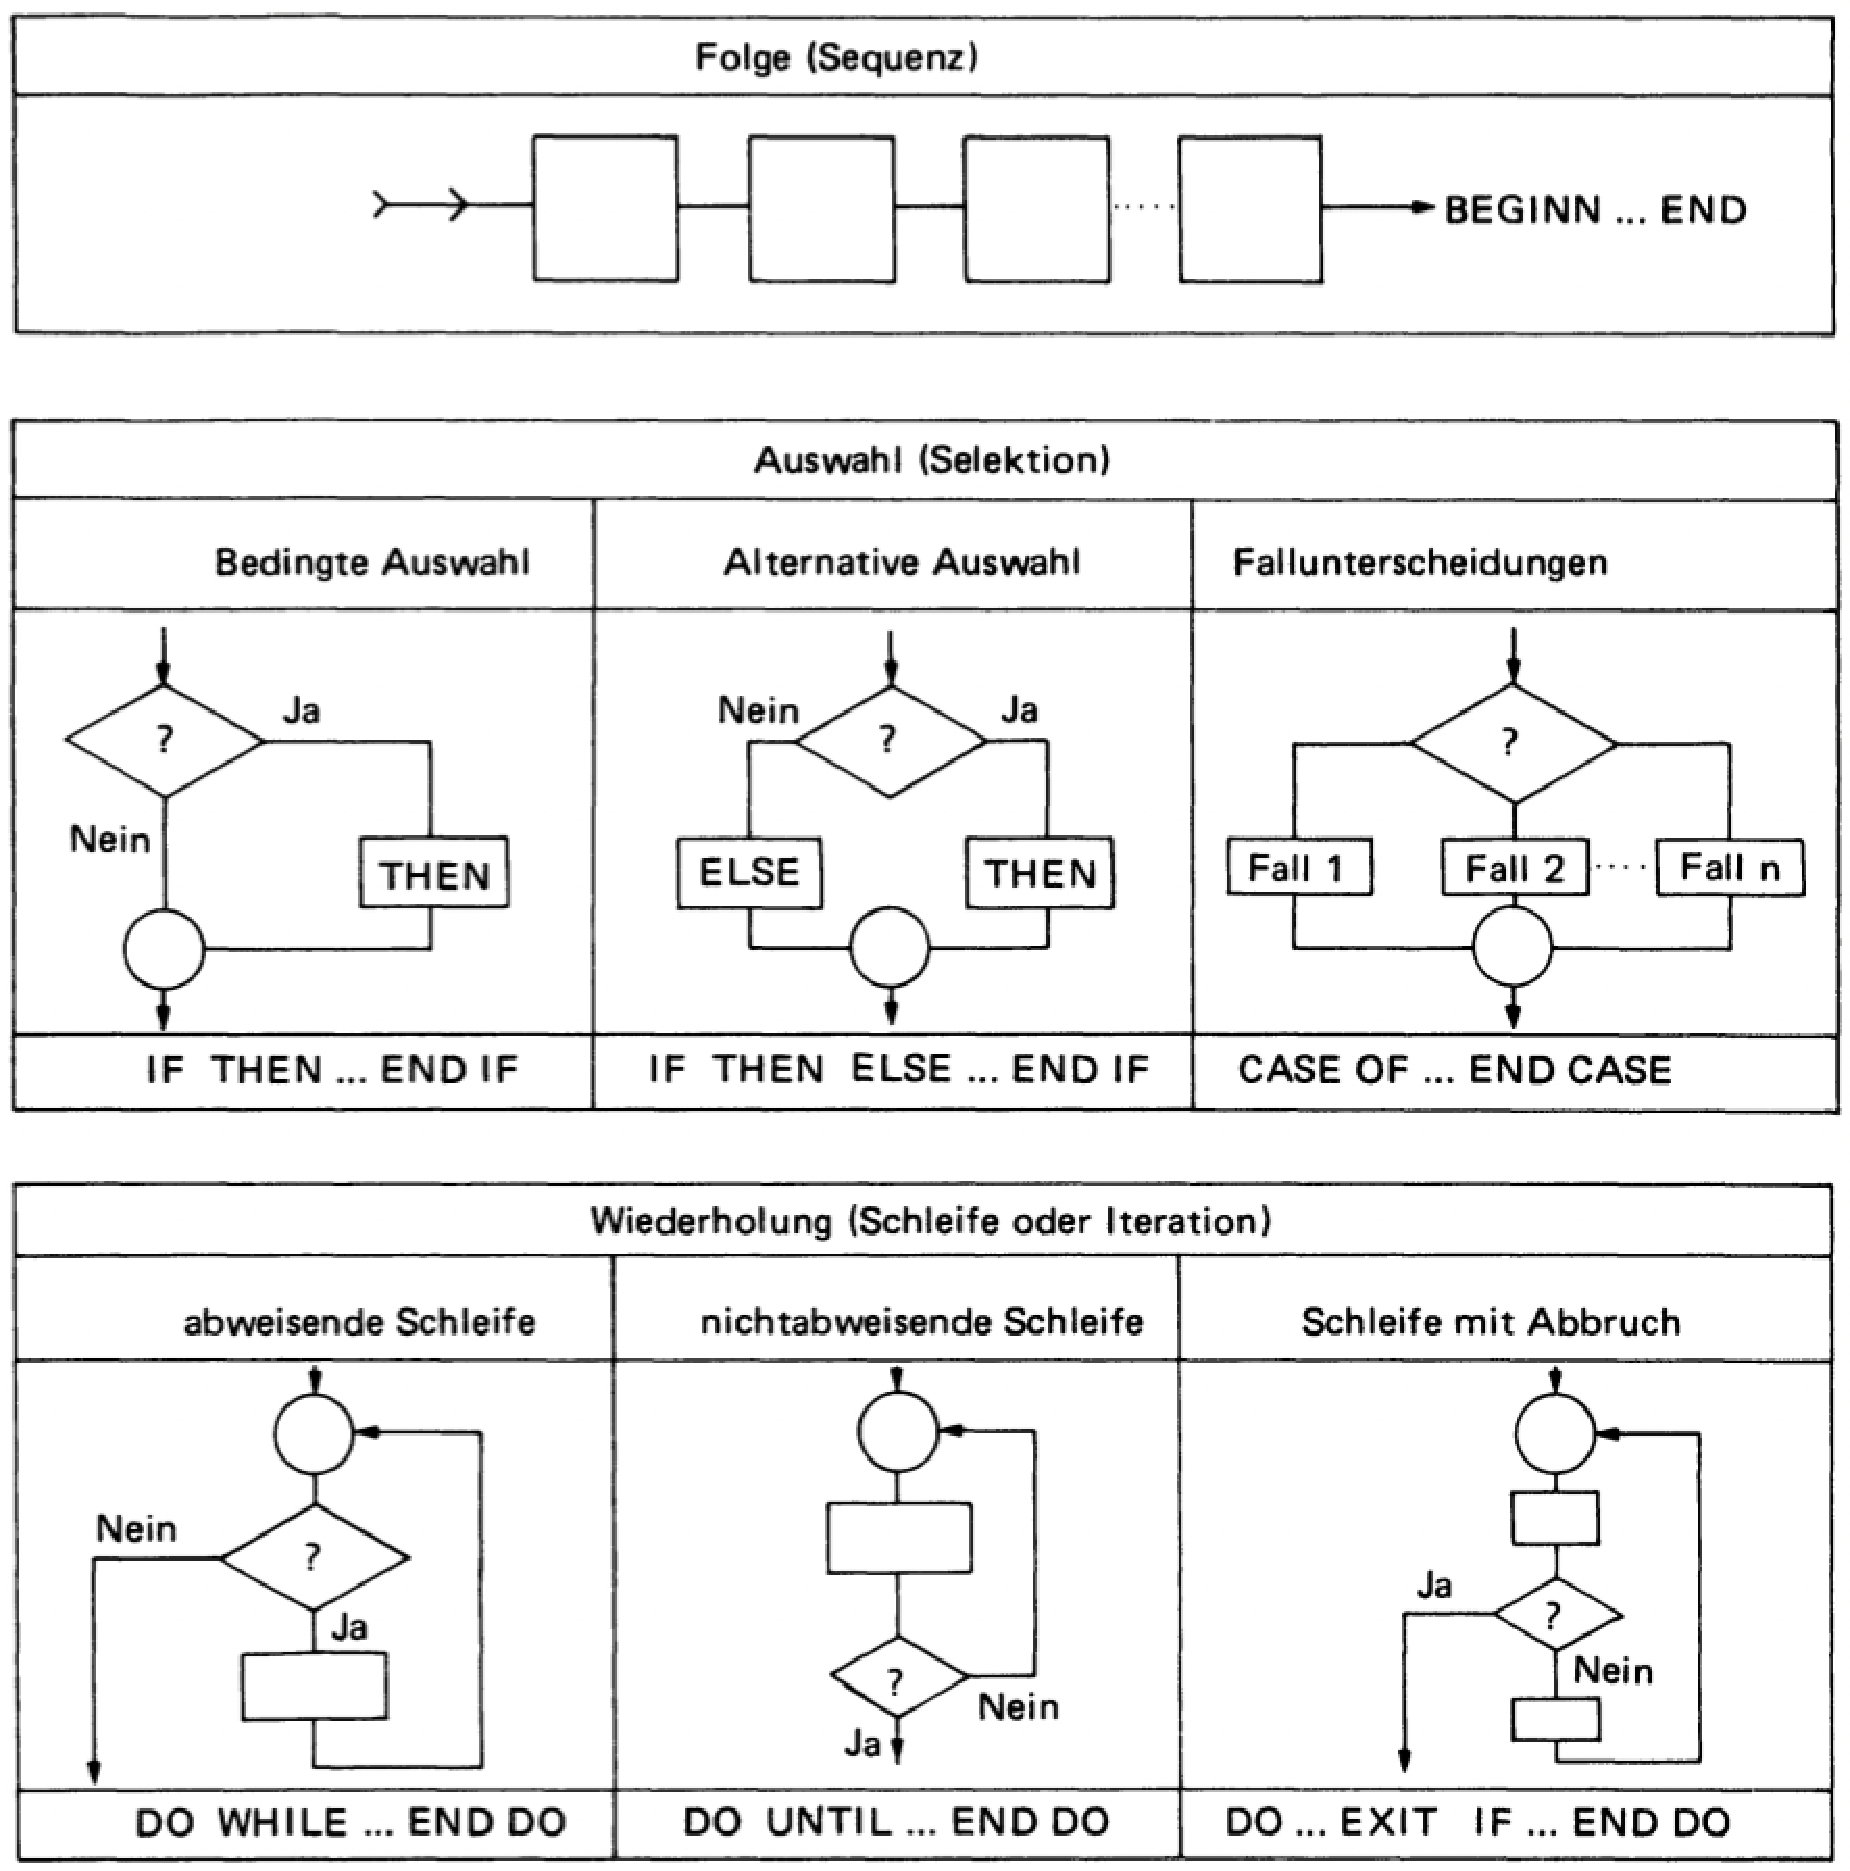
\includegraphics[width=1.0\textwidth]{Bachelorarbeit/images/AnhangUebersichtFlowchart.pdf}
    \caption{Auflistung der elementaren logischen Ablaufstrukturen}
    \label{fig:UebersichtFlowchart}
\end{figure}
\end{document}